\chapter{Supplementary materials for:\\Mapping human health risks from exposure to trace metal contamination of drinking water sources in Pakistan}
\label{appendixD}

\section{Supplementary figures}
\label{Supplementary figures}

See next page.

\begin{landscape}

\begin{figure*}[hp!]
  \centering
  \vspace{-2cm} 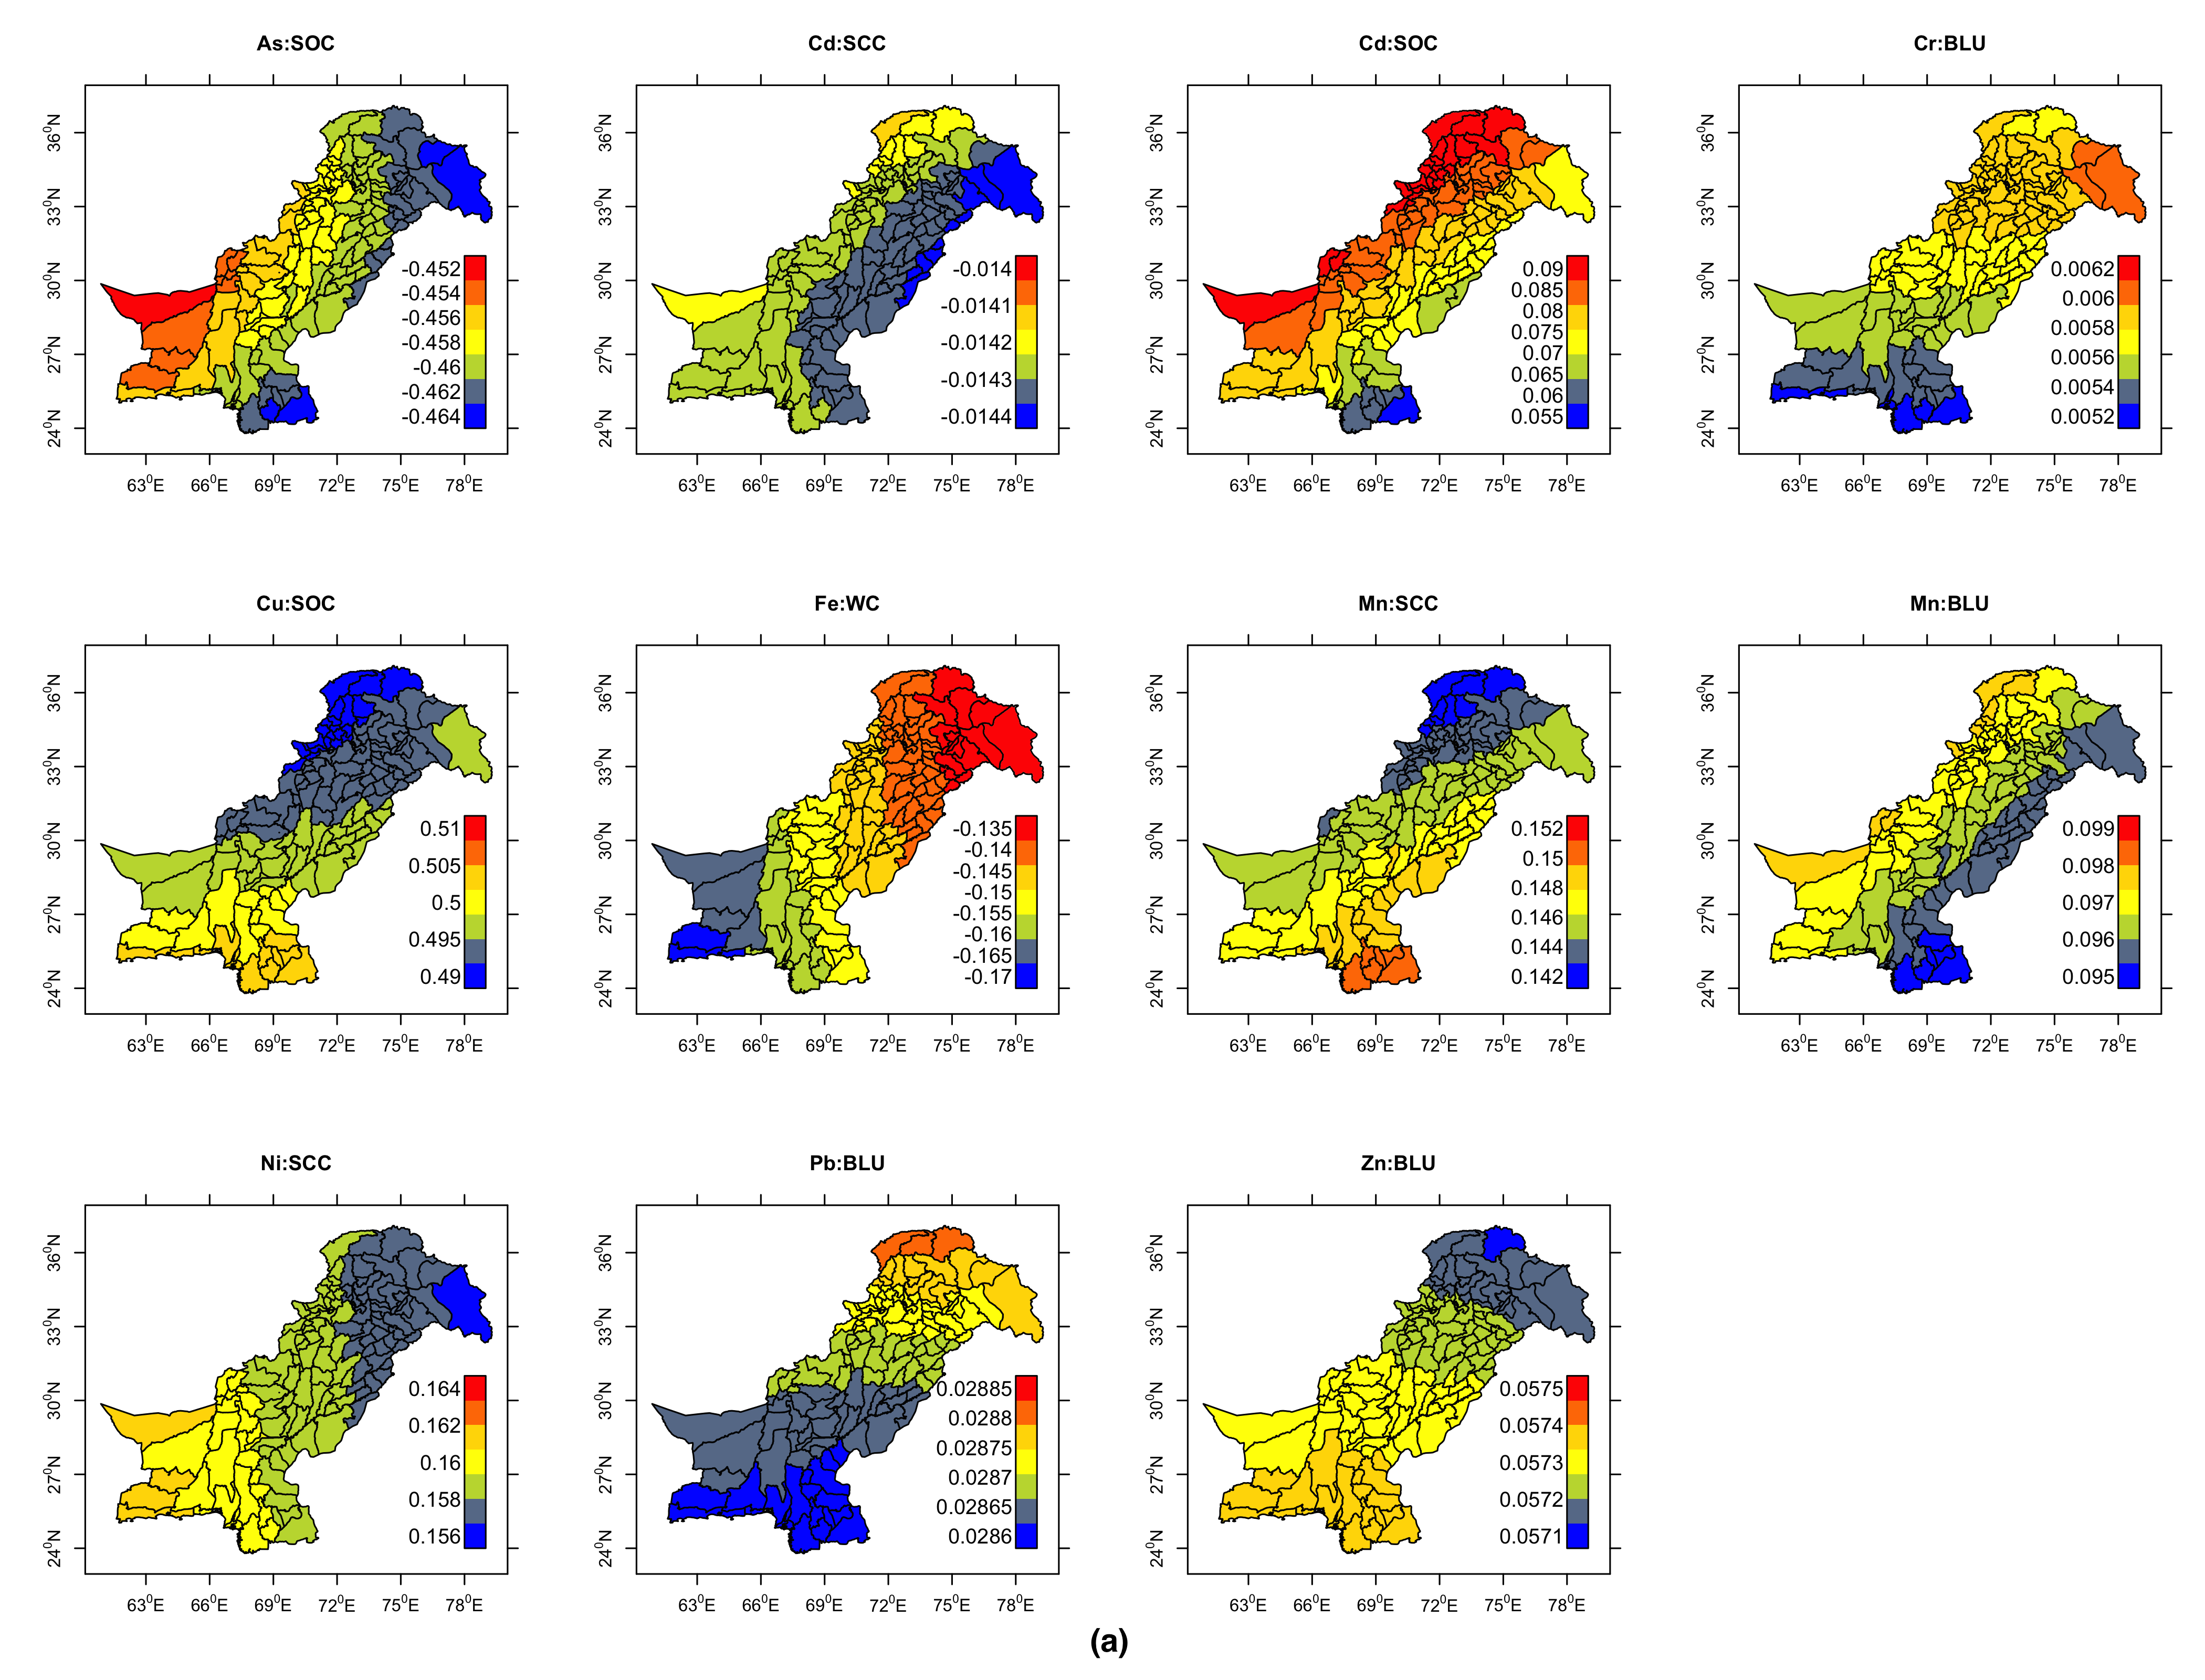
\includegraphics[width=\linewidth]{Figures/Fig_D_1_a.png}
  \label{Fig_D_1_a}
\end{figure*}

\newpage

\begin{figure*}[hp!]
  \centering
  \vspace{-0.5cm} 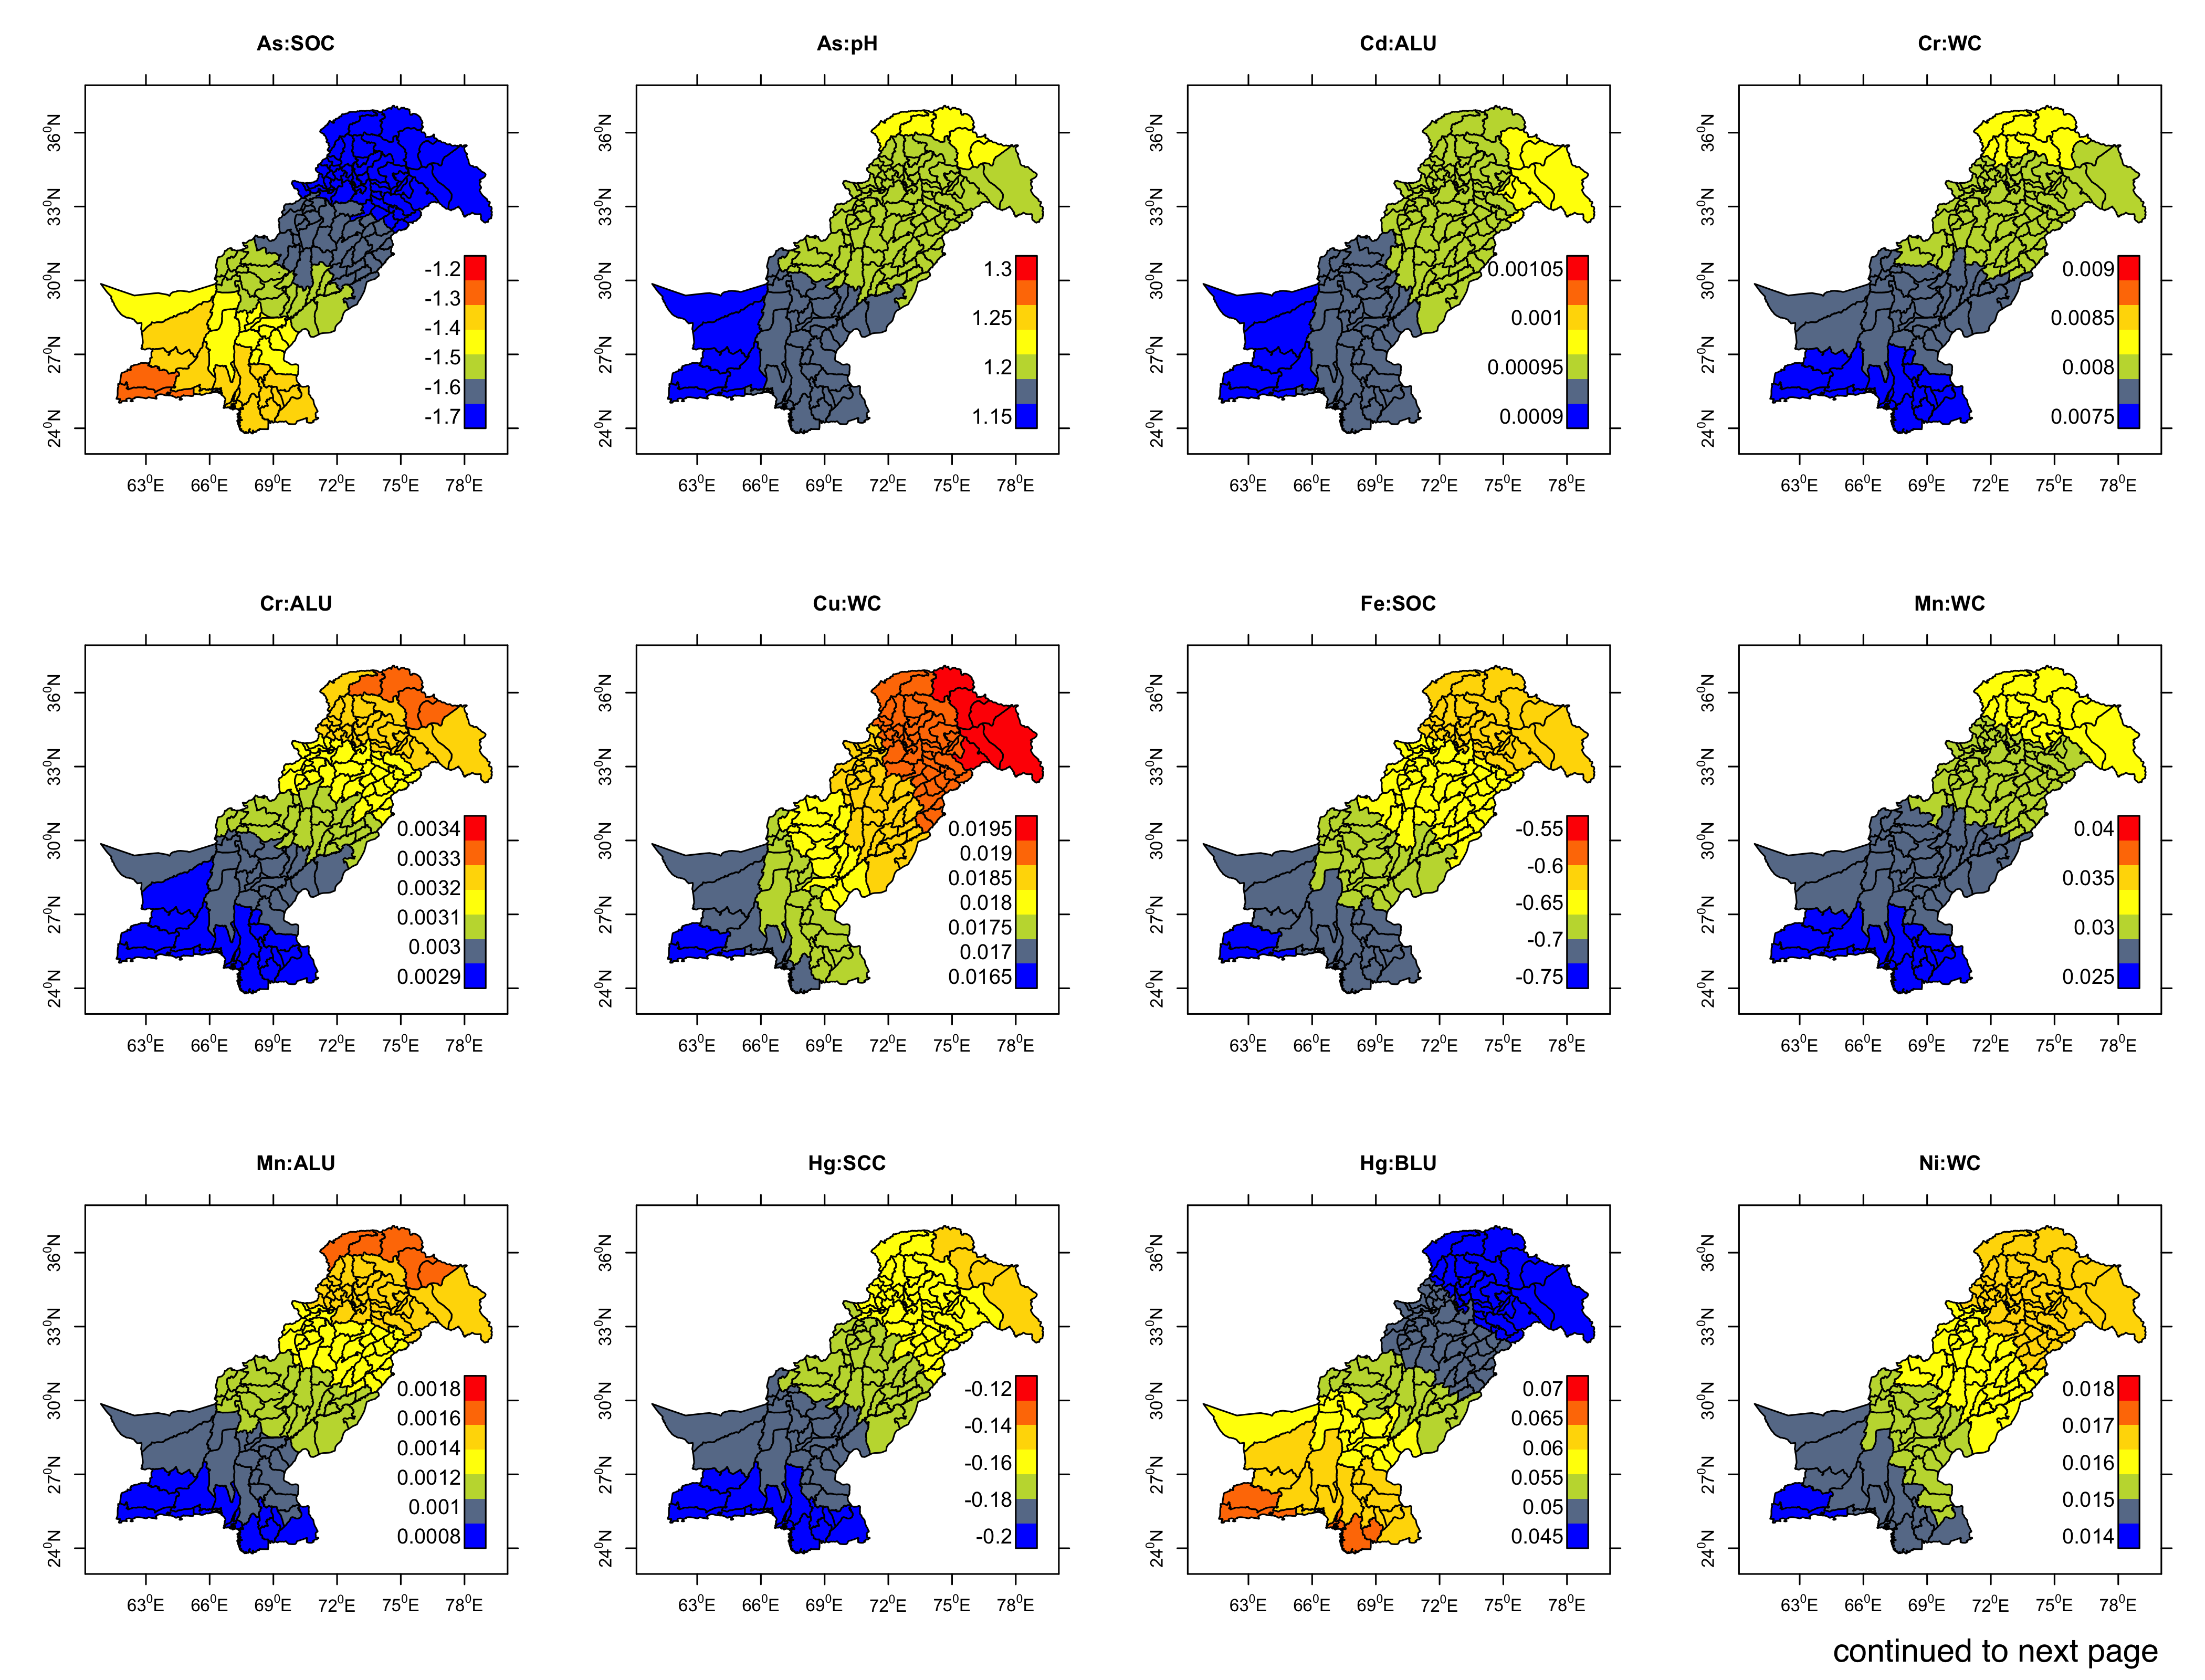
\includegraphics[width=0.95\linewidth]{Figures/Fig_D_1_b_1.png}
  \label{Fig_D_1_b_1}
\end{figure*}

\clearpage

\begin{figure}[h!]
  \centering
  \vspace{-2cm} 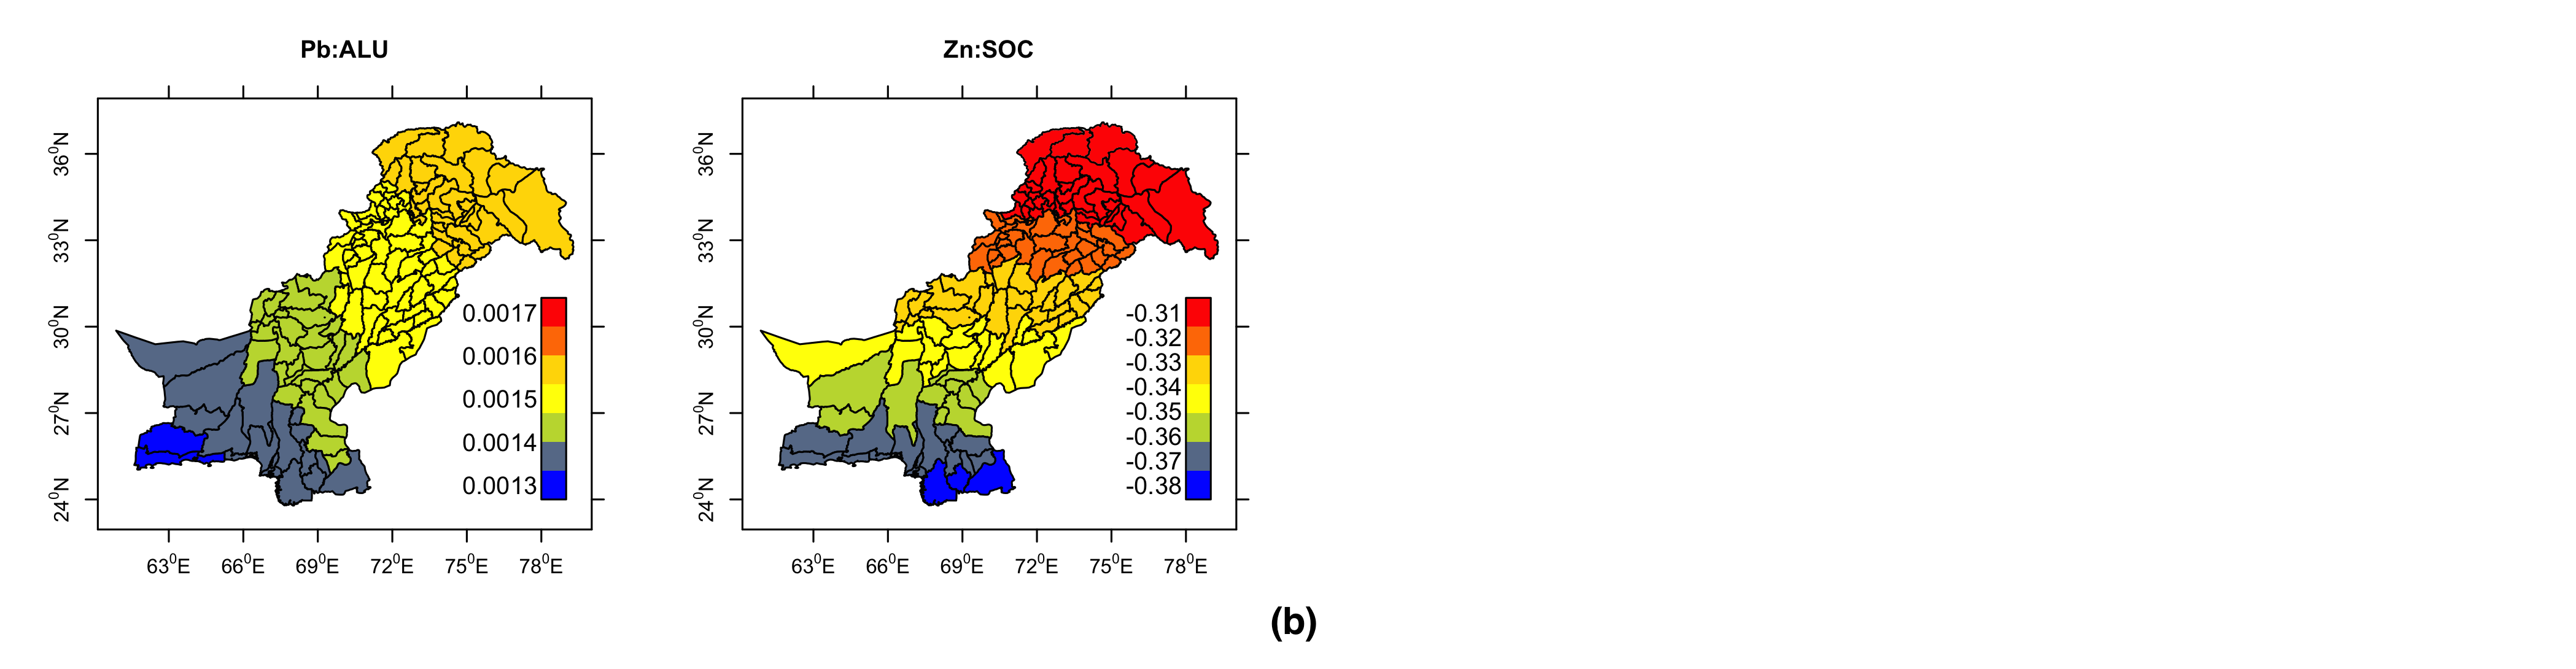
\includegraphics[width=\linewidth]{Figures/Fig_D_1_b_2.png}
  \caption{Geographically weighted regression (GWR) coefficient estimates in each district for the spatial predictors that predicted trace metal concentrations in (a) ground and (b) surface water. The abbreviations used: As = Arsenic, Cd = Cadmium, Cr = Chromium, Cu = Copper, Fe = Iron, Mn = Manganese, Hg = Mercury, Nickel = Ni, Pb = Lead, Zn = Zinc, WC = mean total available water capacity, SOC = mean soil organic carbon density, SCC = mean soil carbonate carbon density, pH= mean soil pH, BLU = percentage of built-up area, ALU = percentage of agricultural area.}
  \label{Fig_D_1_b_2}
\end{figure}

\end{landscape}

\newpage

\begin{figure*}[hp!]
  \centering
  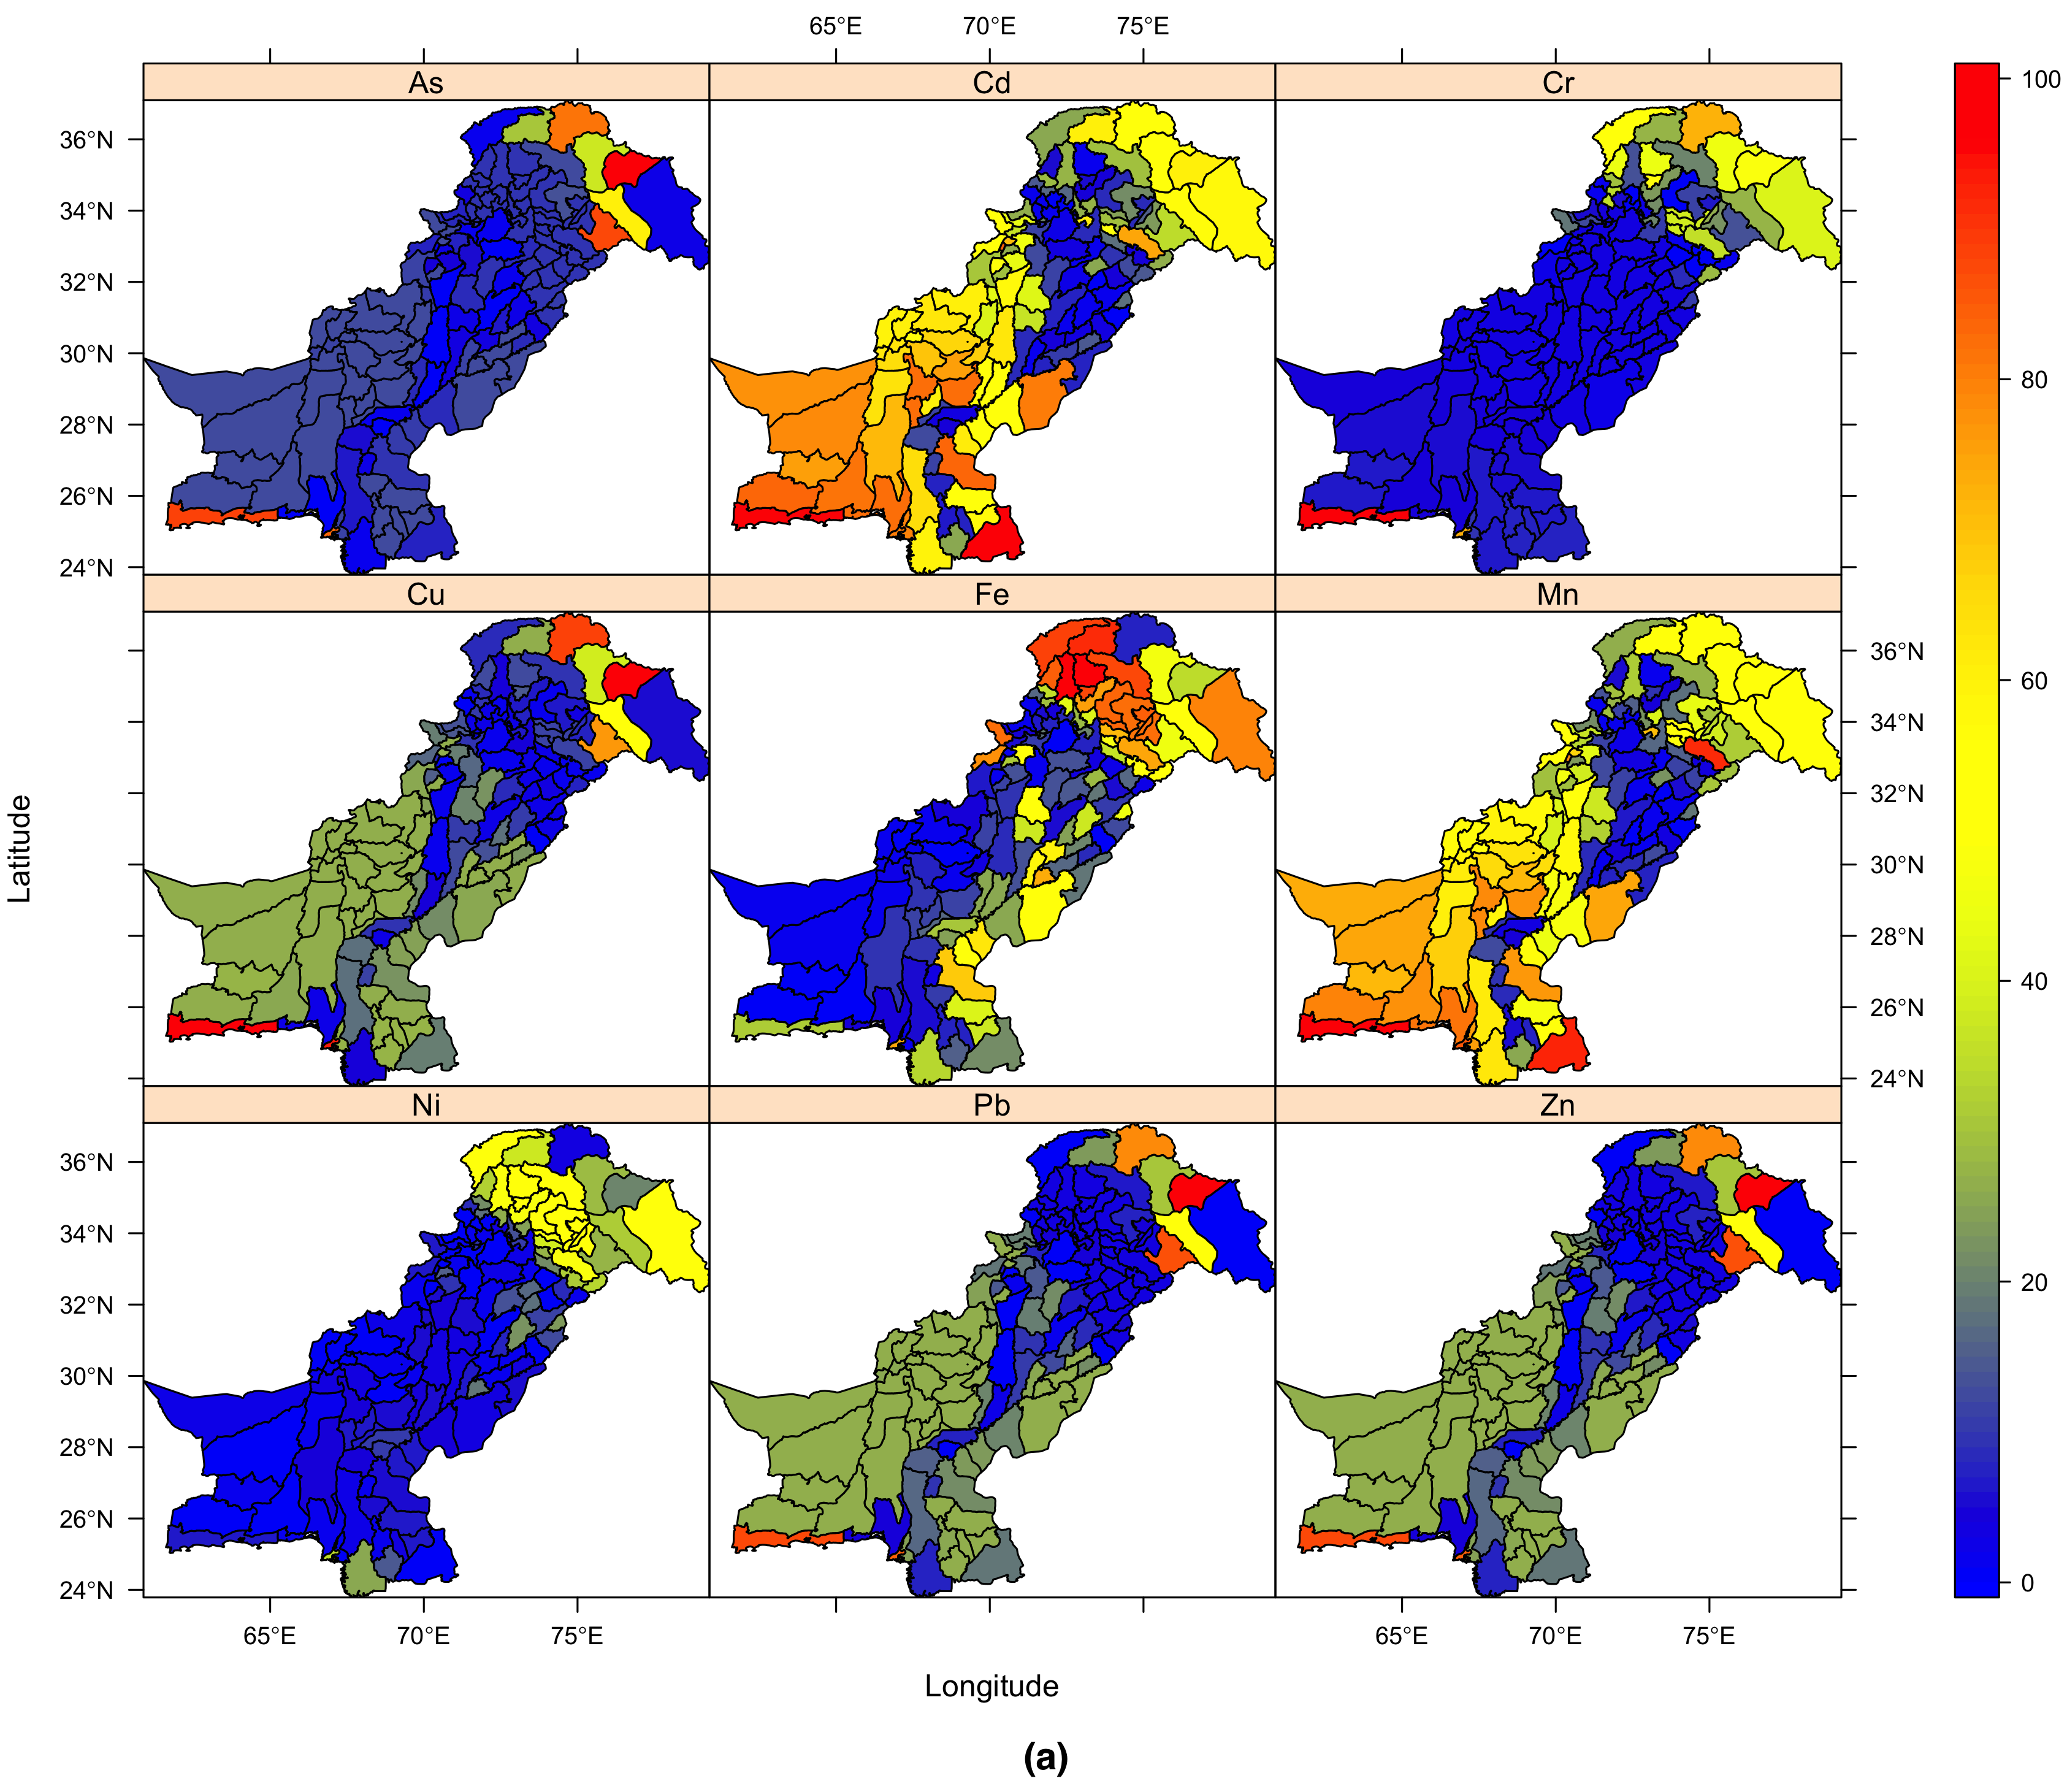
\includegraphics[width=1.1\textwidth]{Figures/Fig_D_2_a.png}
  \label{Fig_D_2_a}
\end{figure*}

\newpage

\begin{landscape}

\begin{figure}[hp!]
  \centering
  \vspace{-2cm} 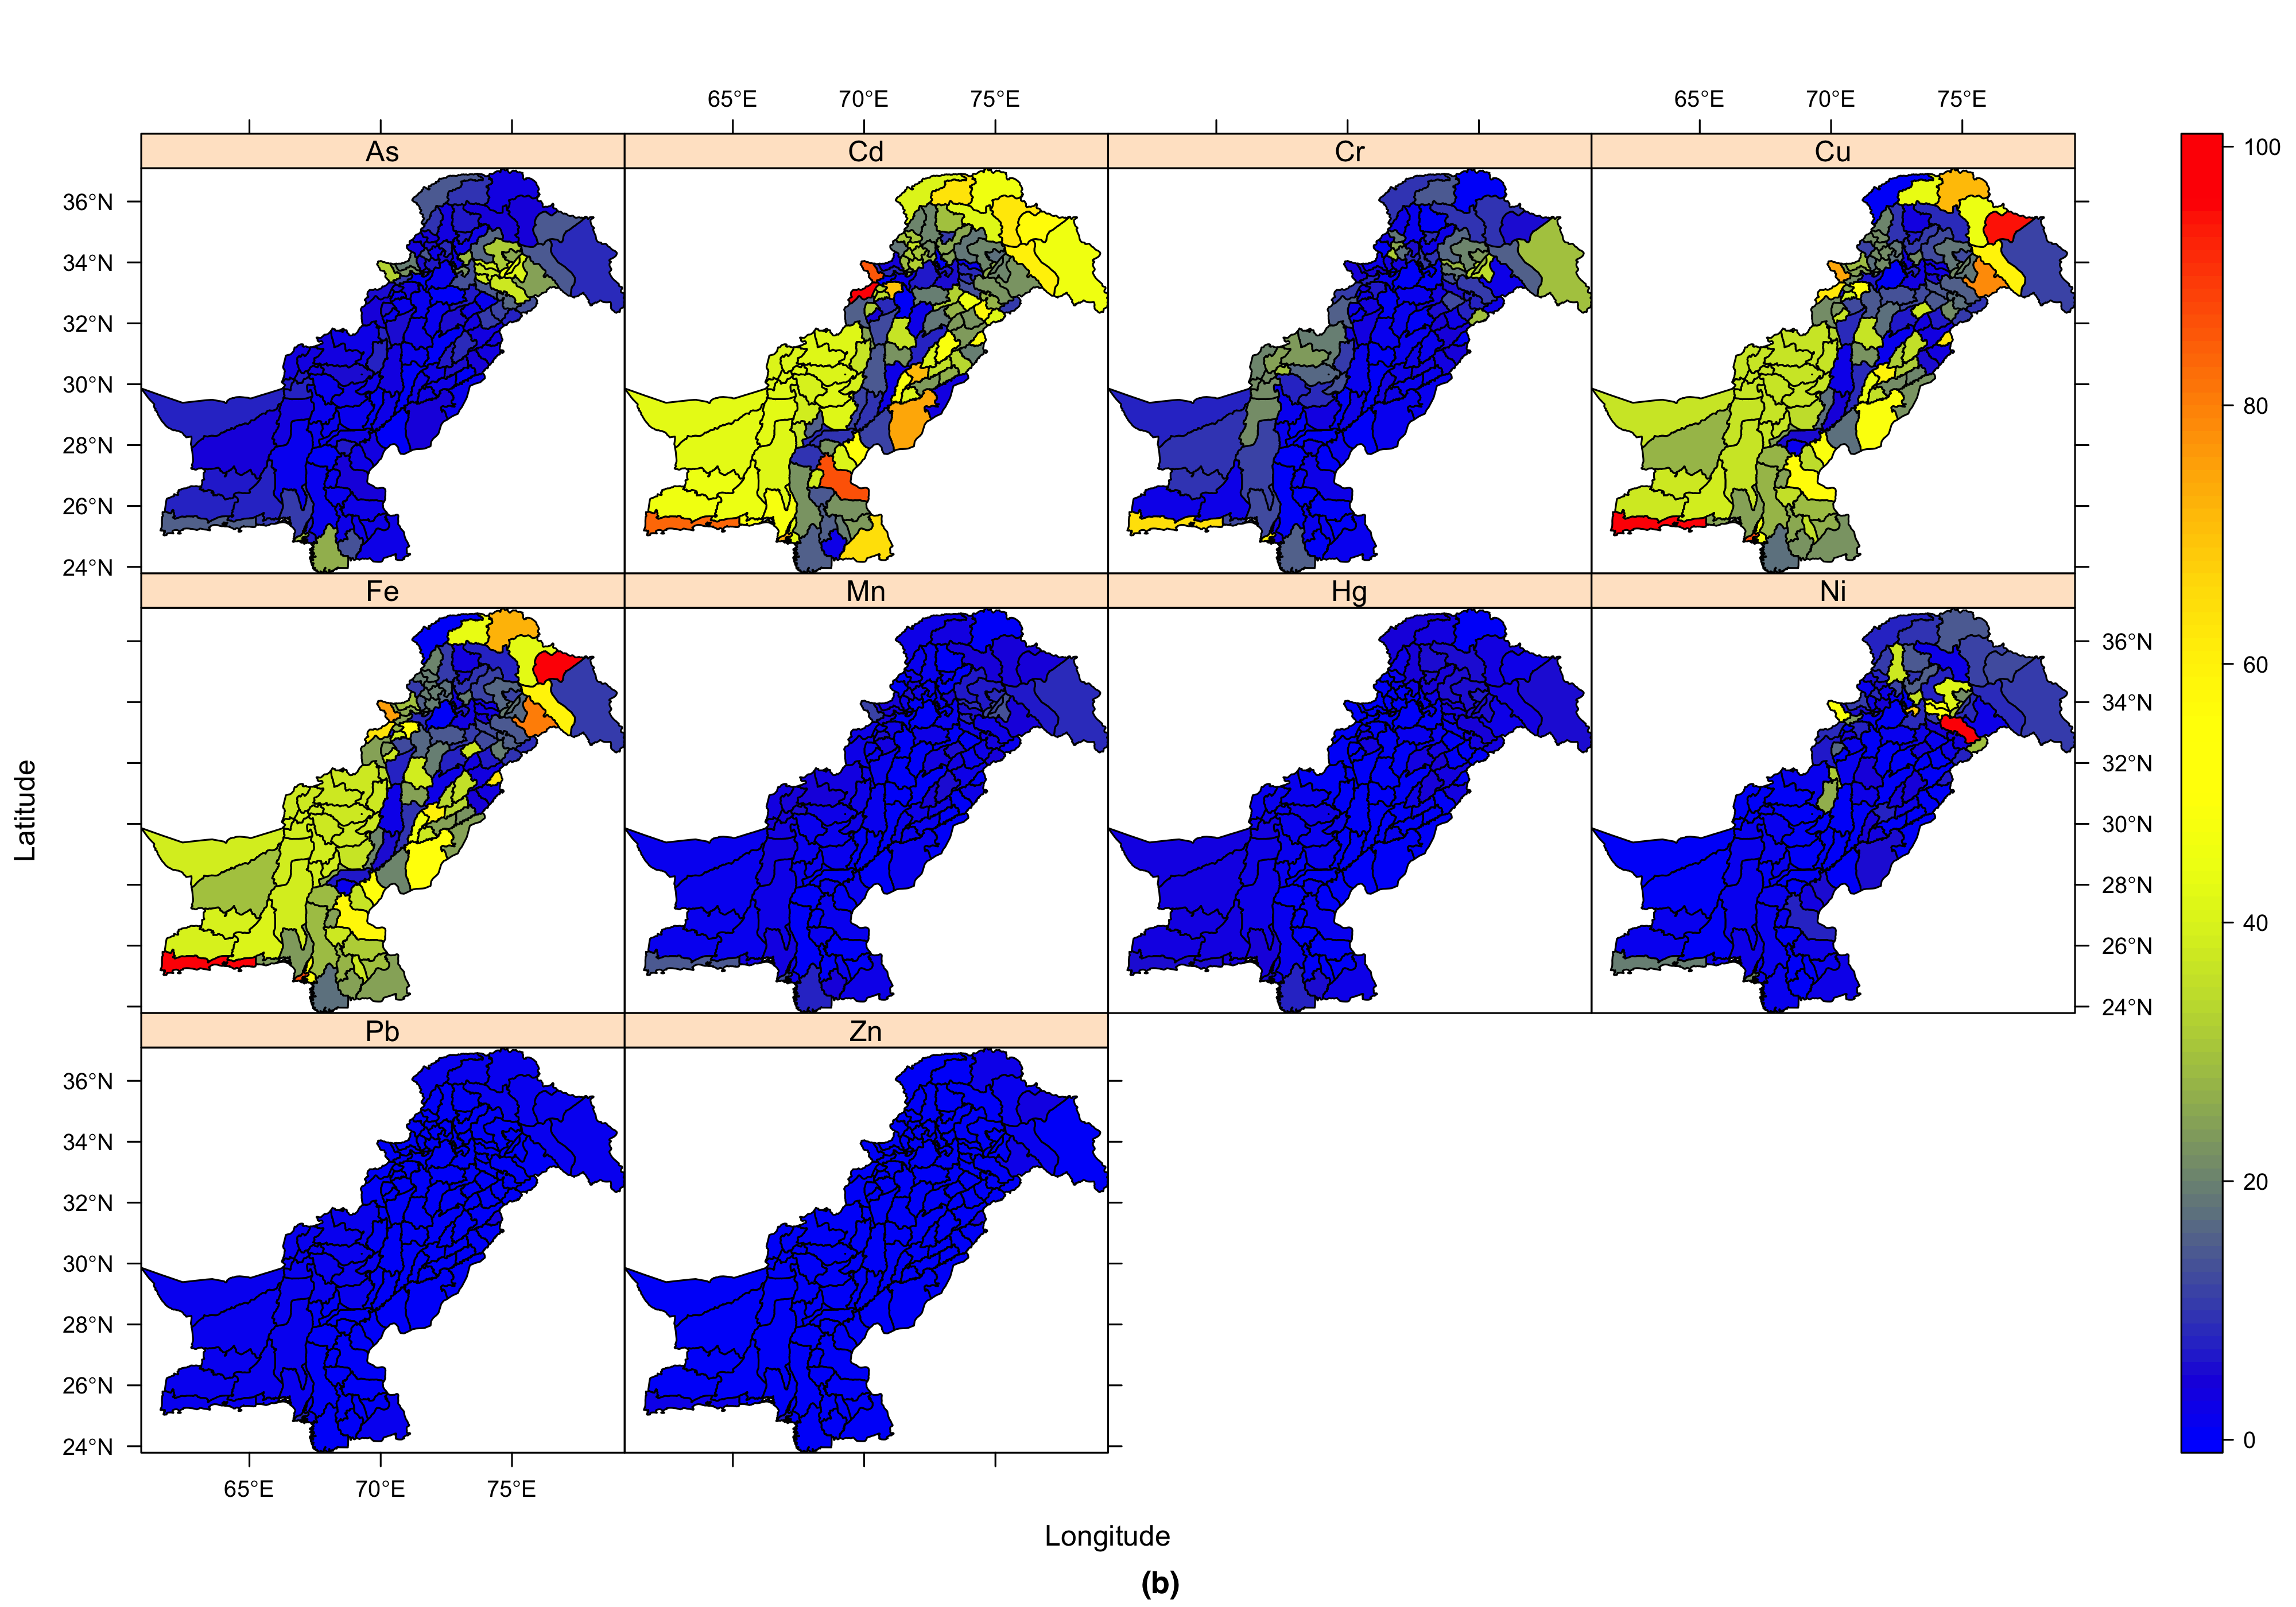
\includegraphics[width=\linewidth]{Figures/Fig_D_2_b.png}
  \caption{GWR prediction standard errors (in \%) for prediction of trace metal concentrations in (a) ground and (b) surface water of each district. The abbreviations used: As = Arsenic, Cd = Cadmium, Cr = Chromium, Cu = Copper, Fe = Iron, Mn = Manganese, Hg = Mercury, Nickel = Ni, Pb = Lead, Zn = Zinc.}
  \label{Fig_D_2_b}
\end{figure}

\end{landscape}

\newpage

\begin{figure*}[hp!]
  \centering
  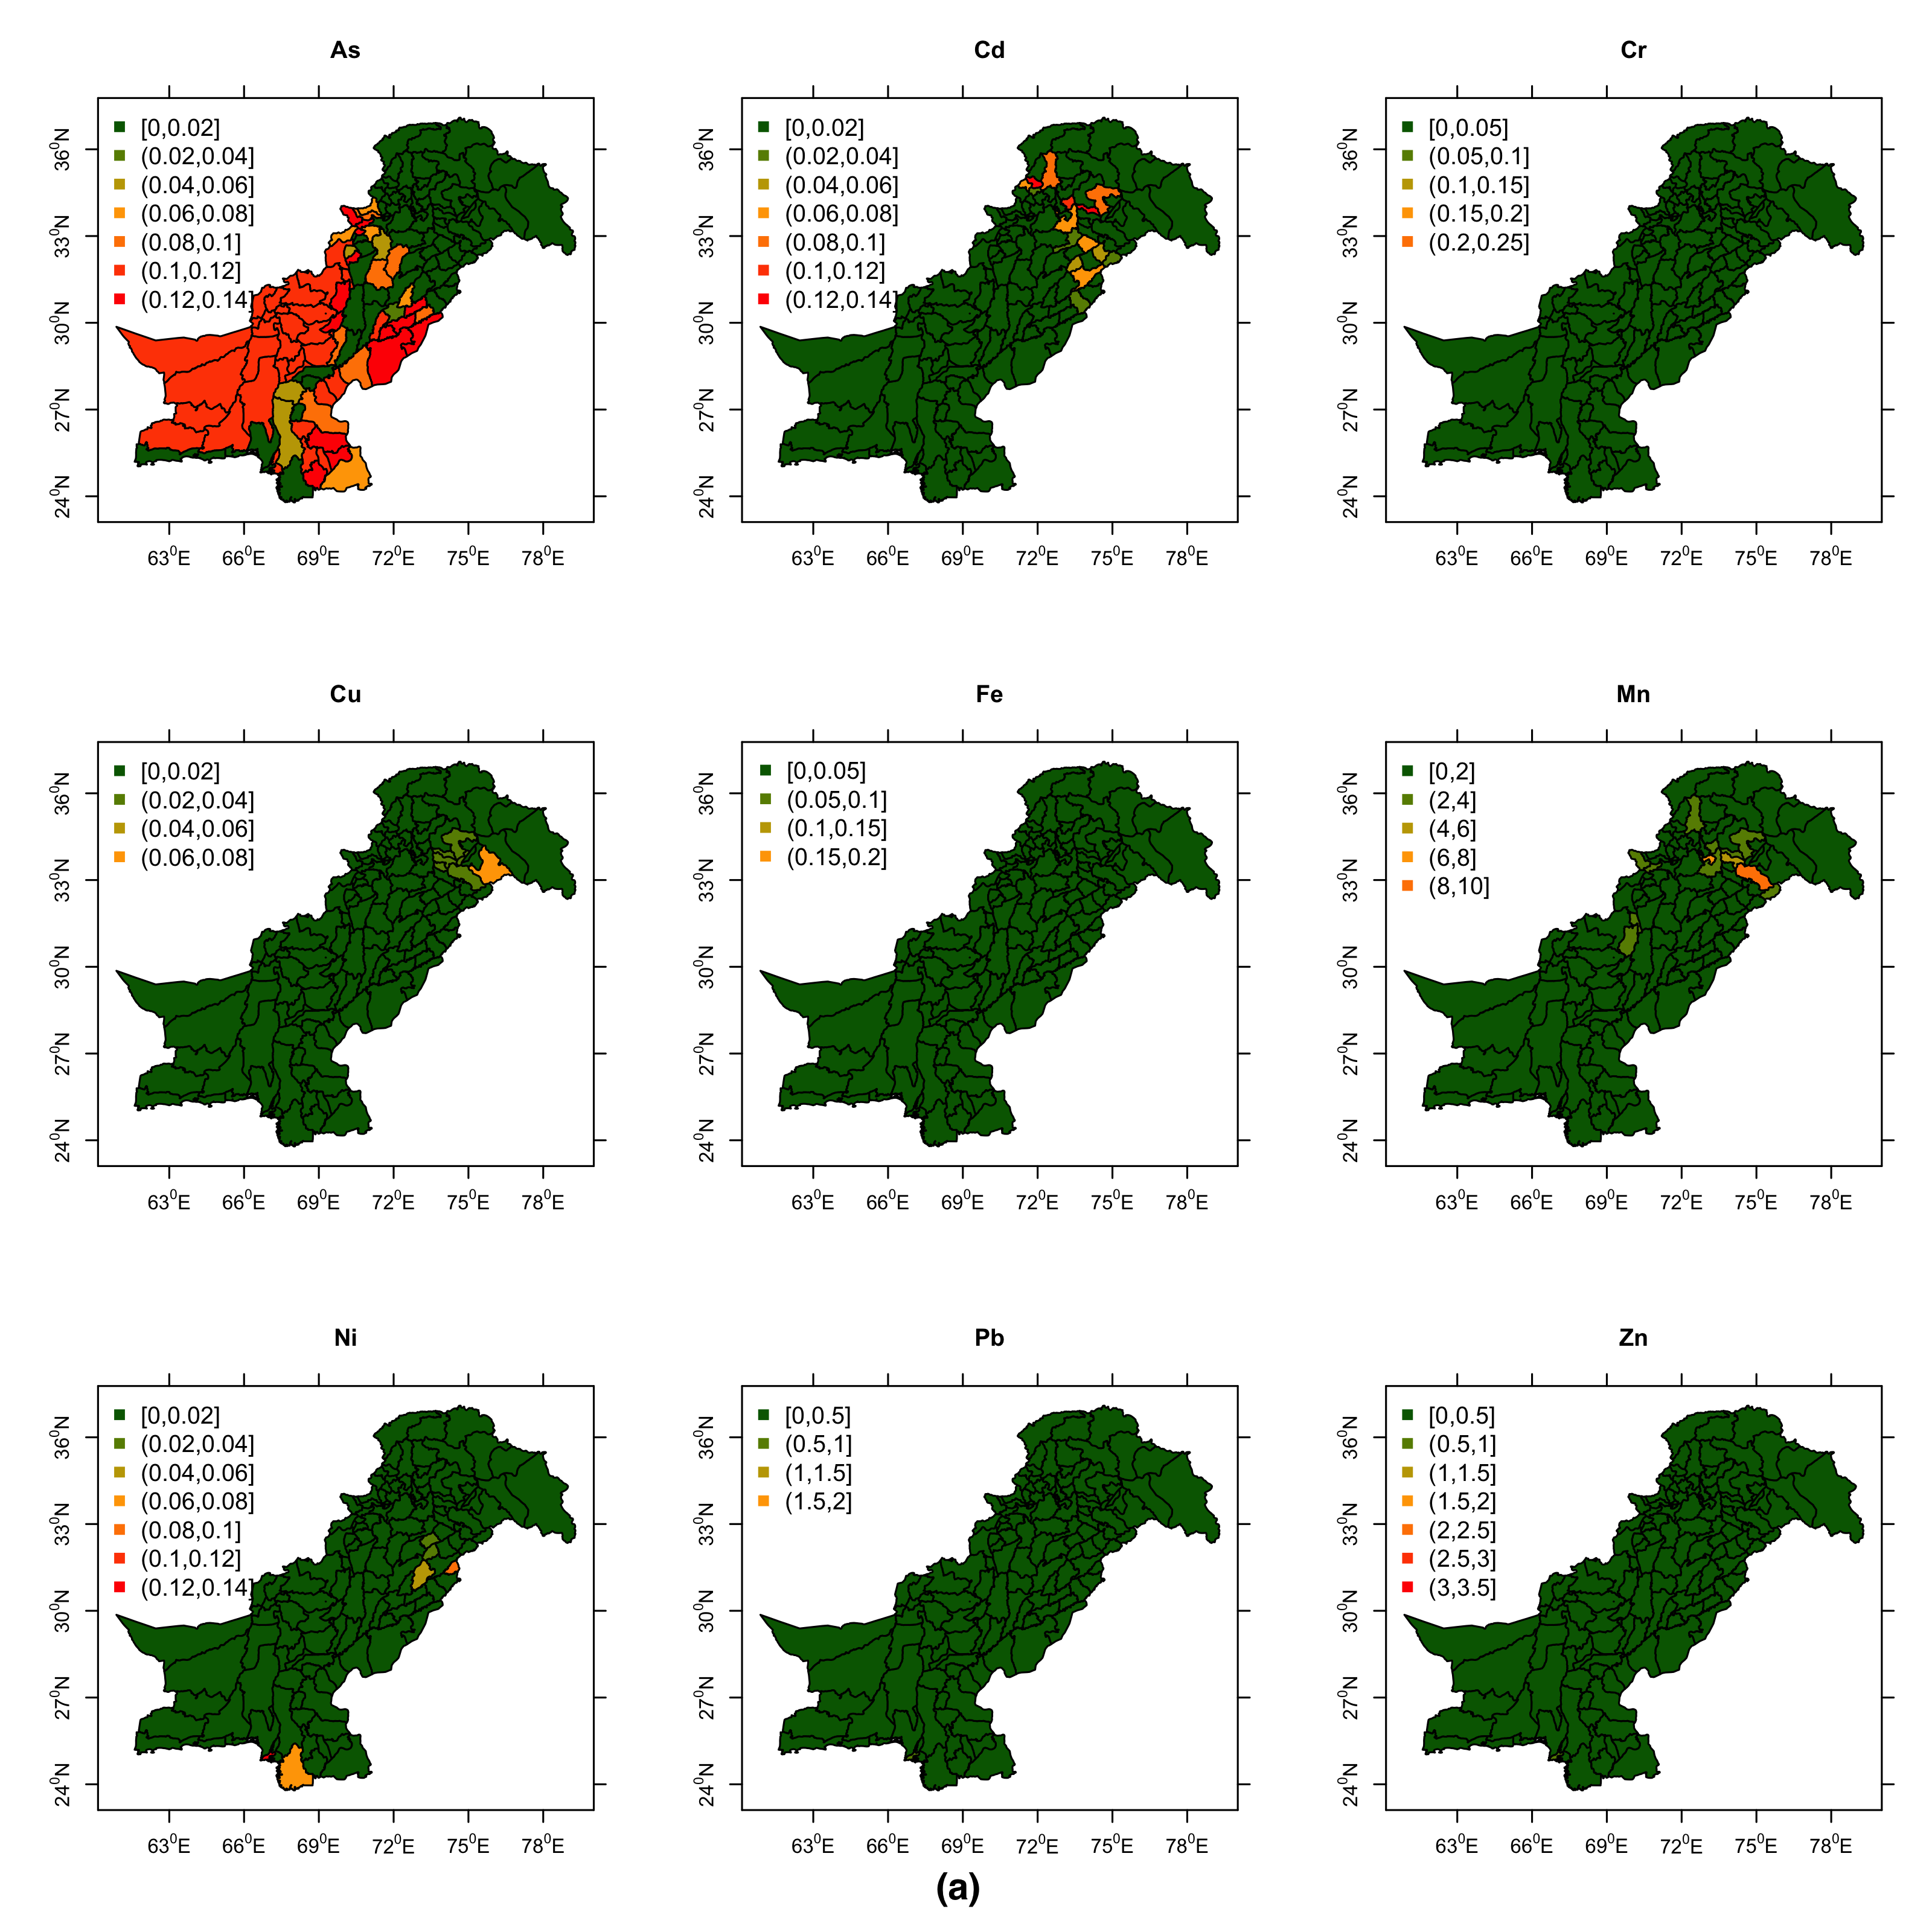
\includegraphics[width=1.1\textwidth]{Figures/Fig_D_3_a.png}
  \label{Fig_D_3_a}
\end{figure*}

\newpage

\begin{landscape}

\begin{figure}[hp!]
  \centering
  \vspace{-2.5cm} 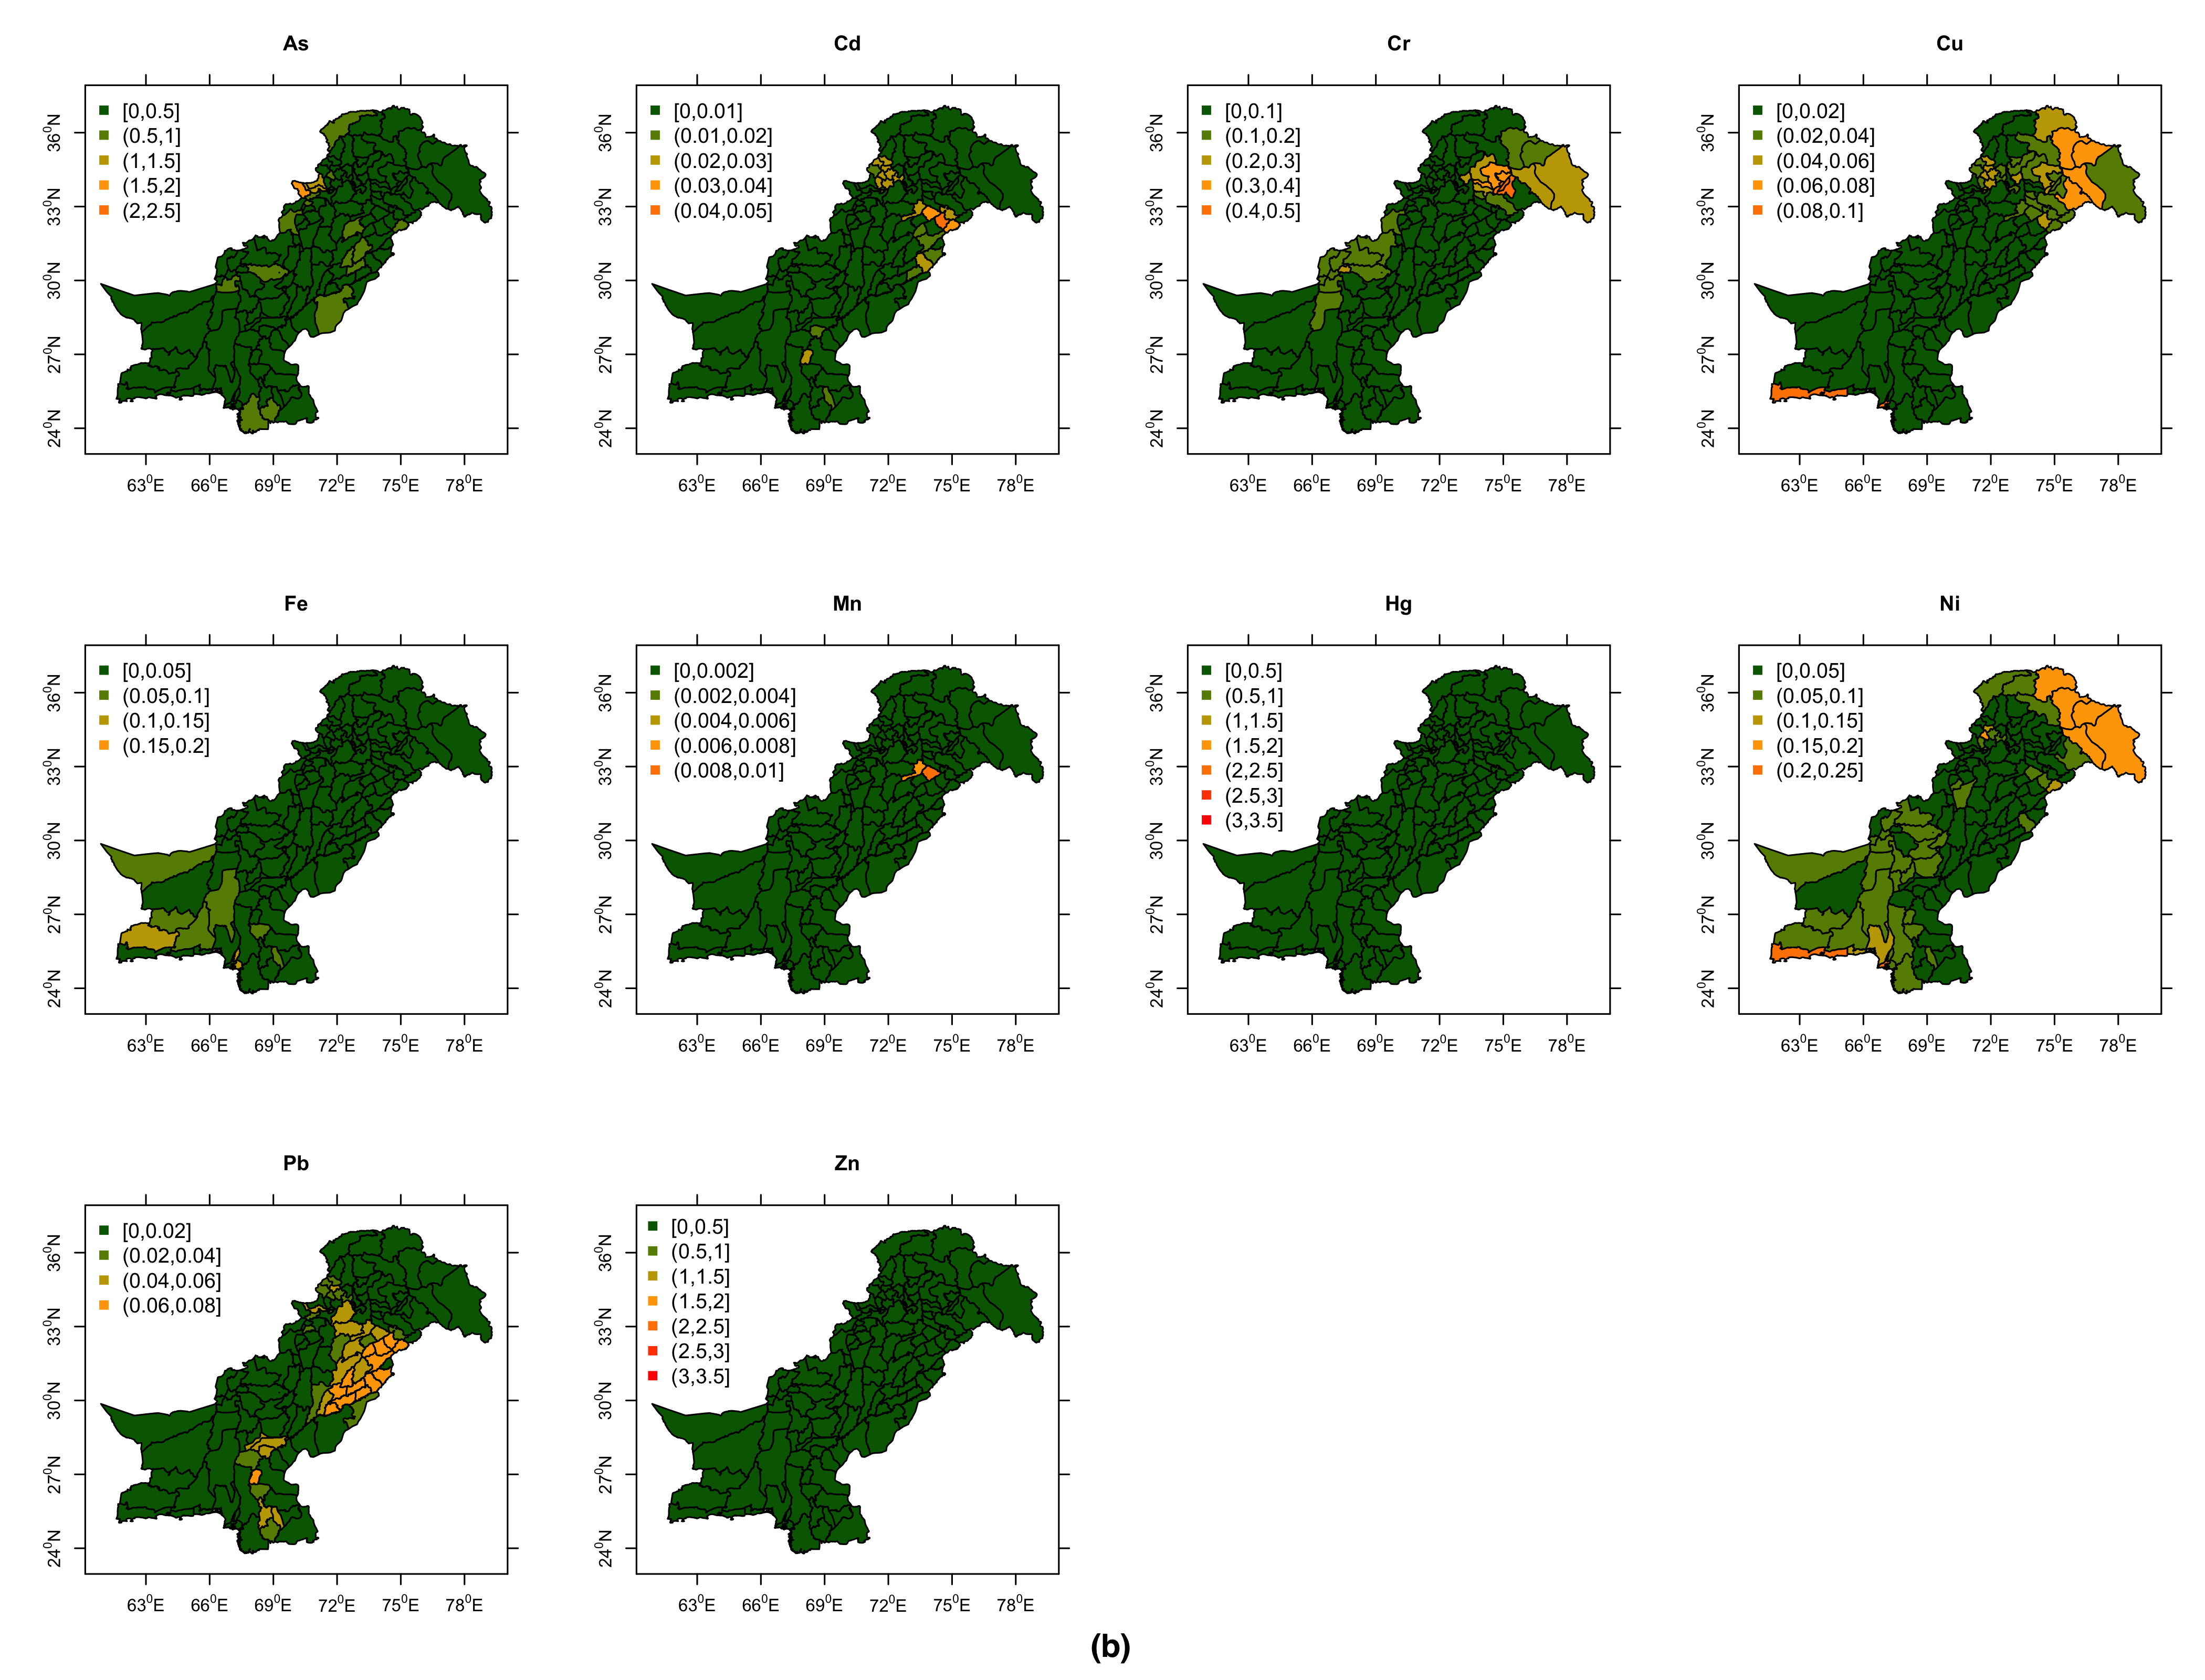
\includegraphics[width=\linewidth]{Figures/Fig_D_3_b.png}
  \caption{Lower confidence boundaries of GWR model predicted trace metal concentrations (in mg / l) within 95 \% confidence interval, i.e. predicted concentrations – 1.96 * standard errors, in (a) ground and (b) surface water at the districts of Pakistan.  The abbreviations used: As = Arsenic, Cd = Cadmium, Cr = Chromium, Cu = Copper, Fe = Iron, Mn = Manganese, Hg = Mercury, Nickel = Ni, Pb = Lead, Zn = Zinc.}
  \label{Fig_D_3_b}
\end{figure}

\end{landscape}

\newpage

\begin{figure*}[hp!]
  \centering
  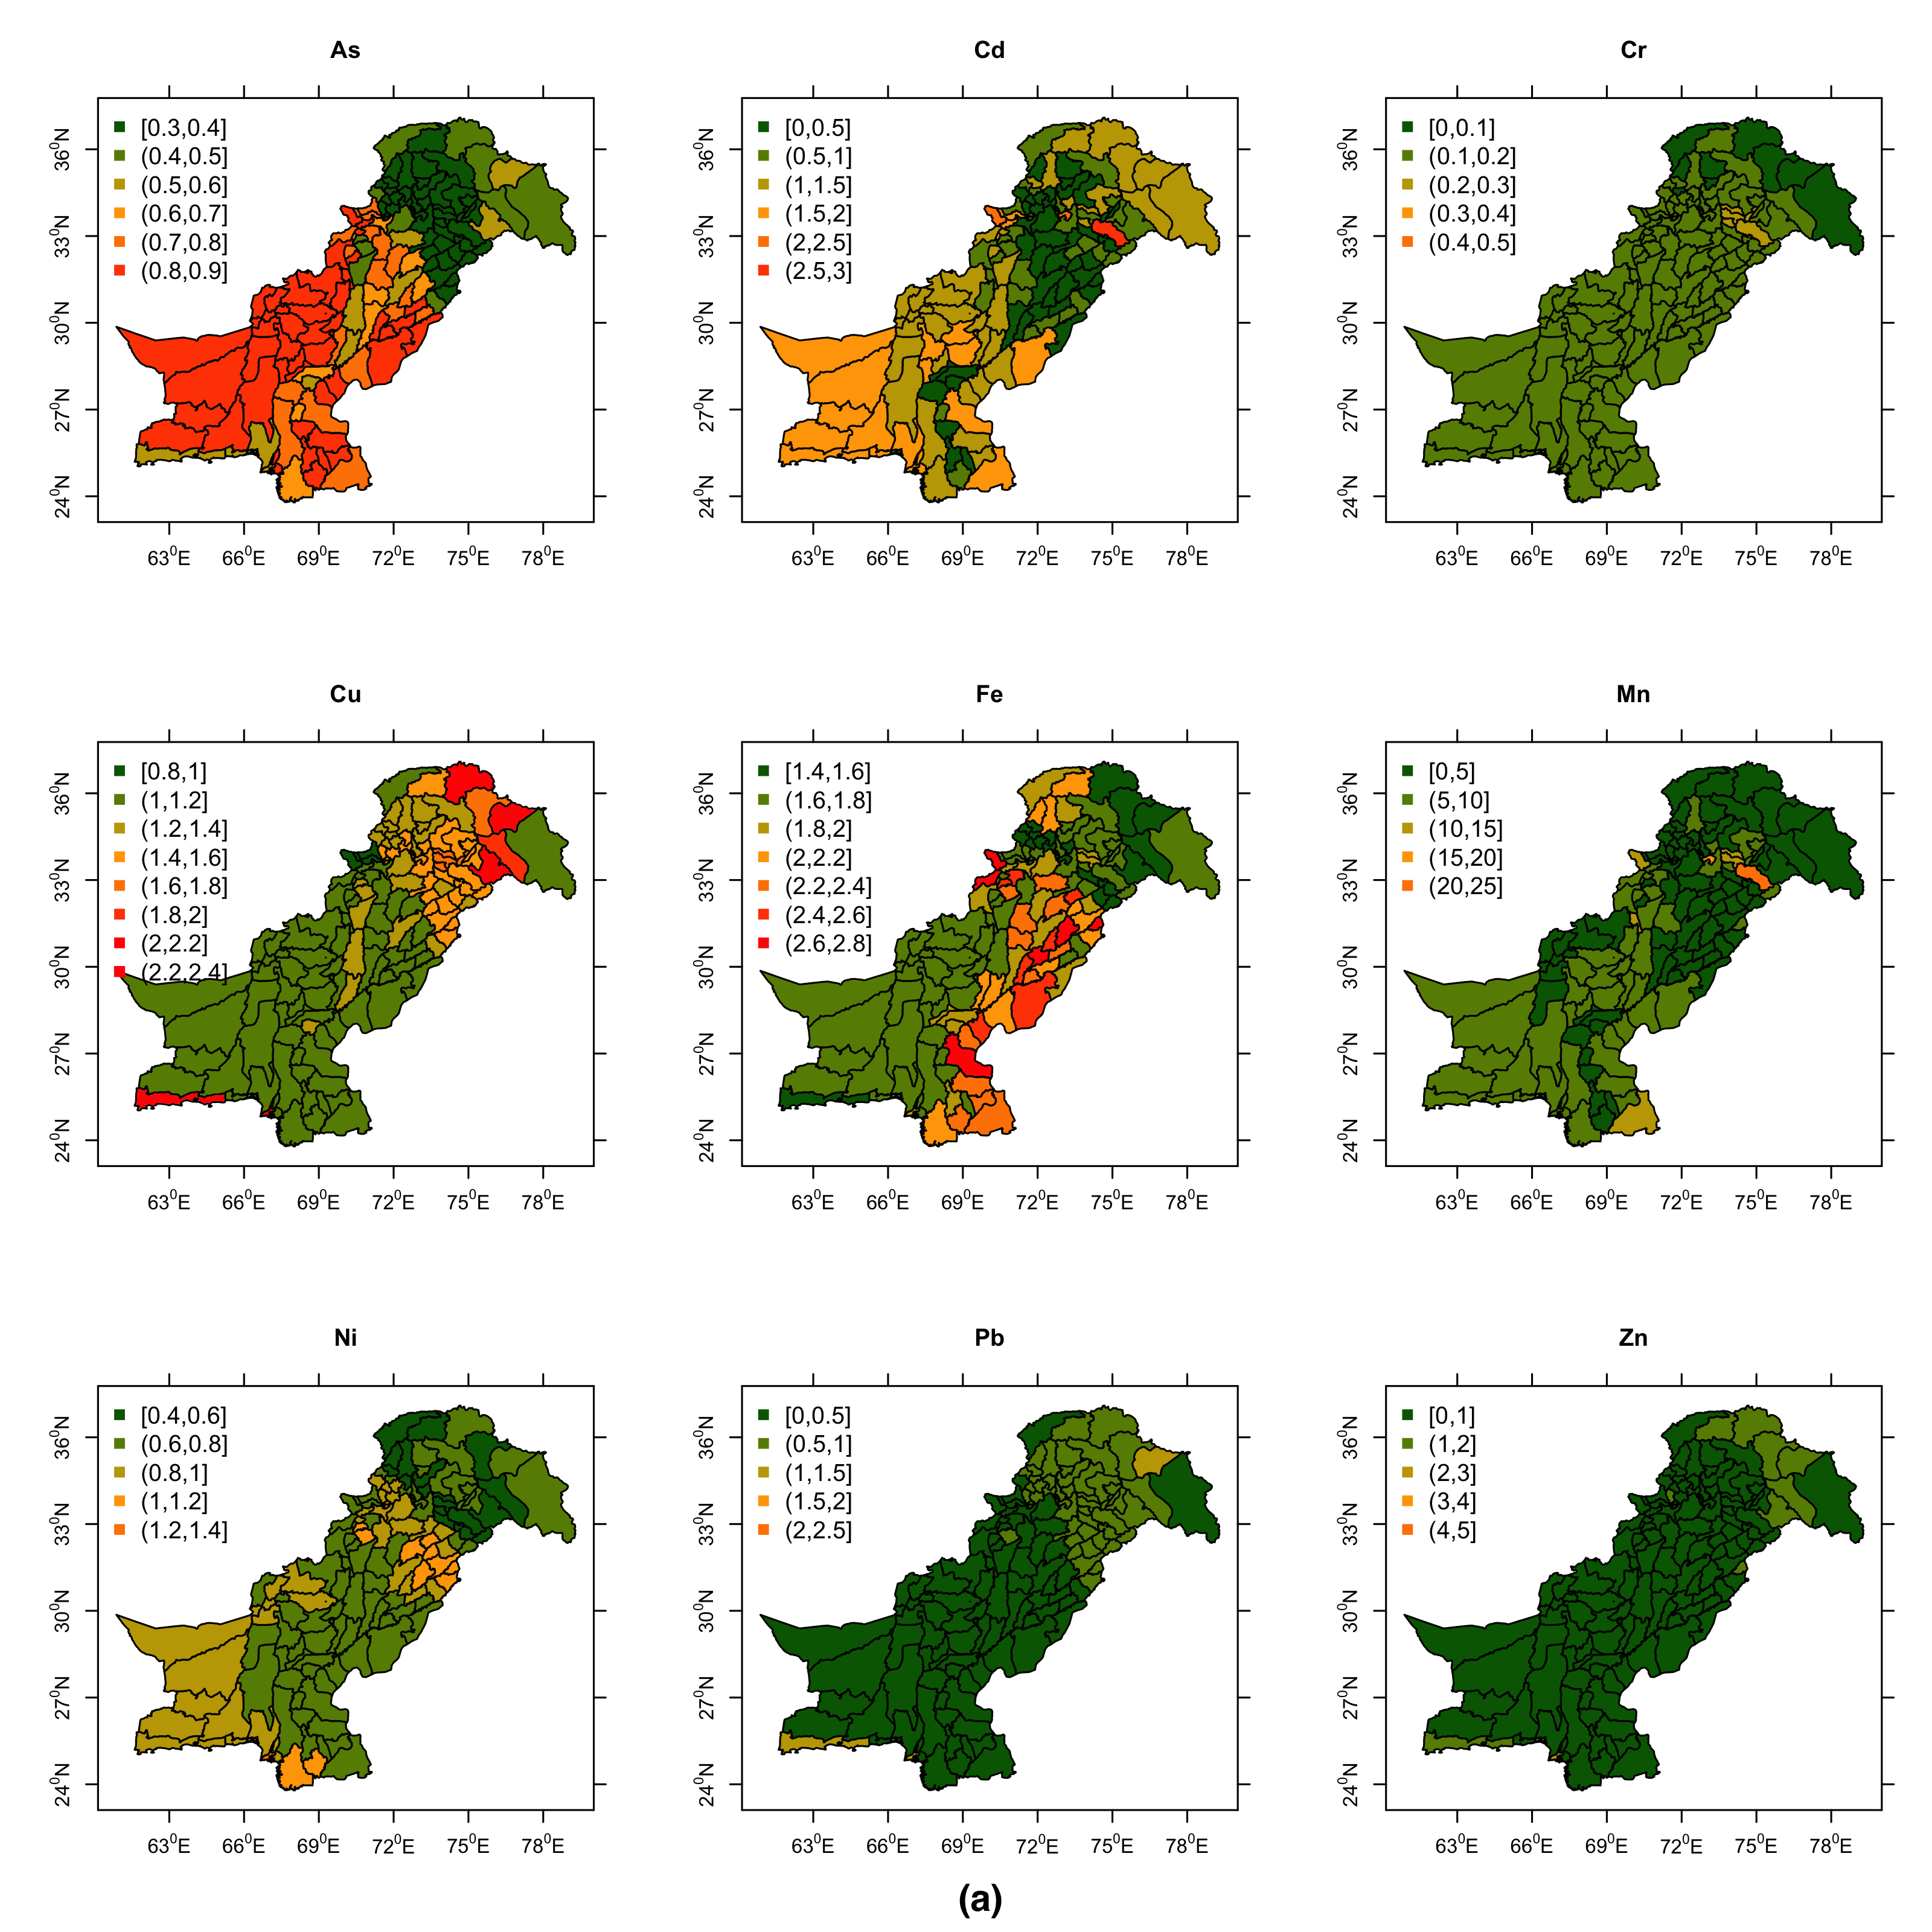
\includegraphics[width=1.1\textwidth]{Figures/Fig_D_4_a.png}
  \label{Fig_D_4_a}
\end{figure*}

\newpage

\begin{landscape}

\begin{figure}[hp!]
  \centering
  \vspace{-2.5cm} 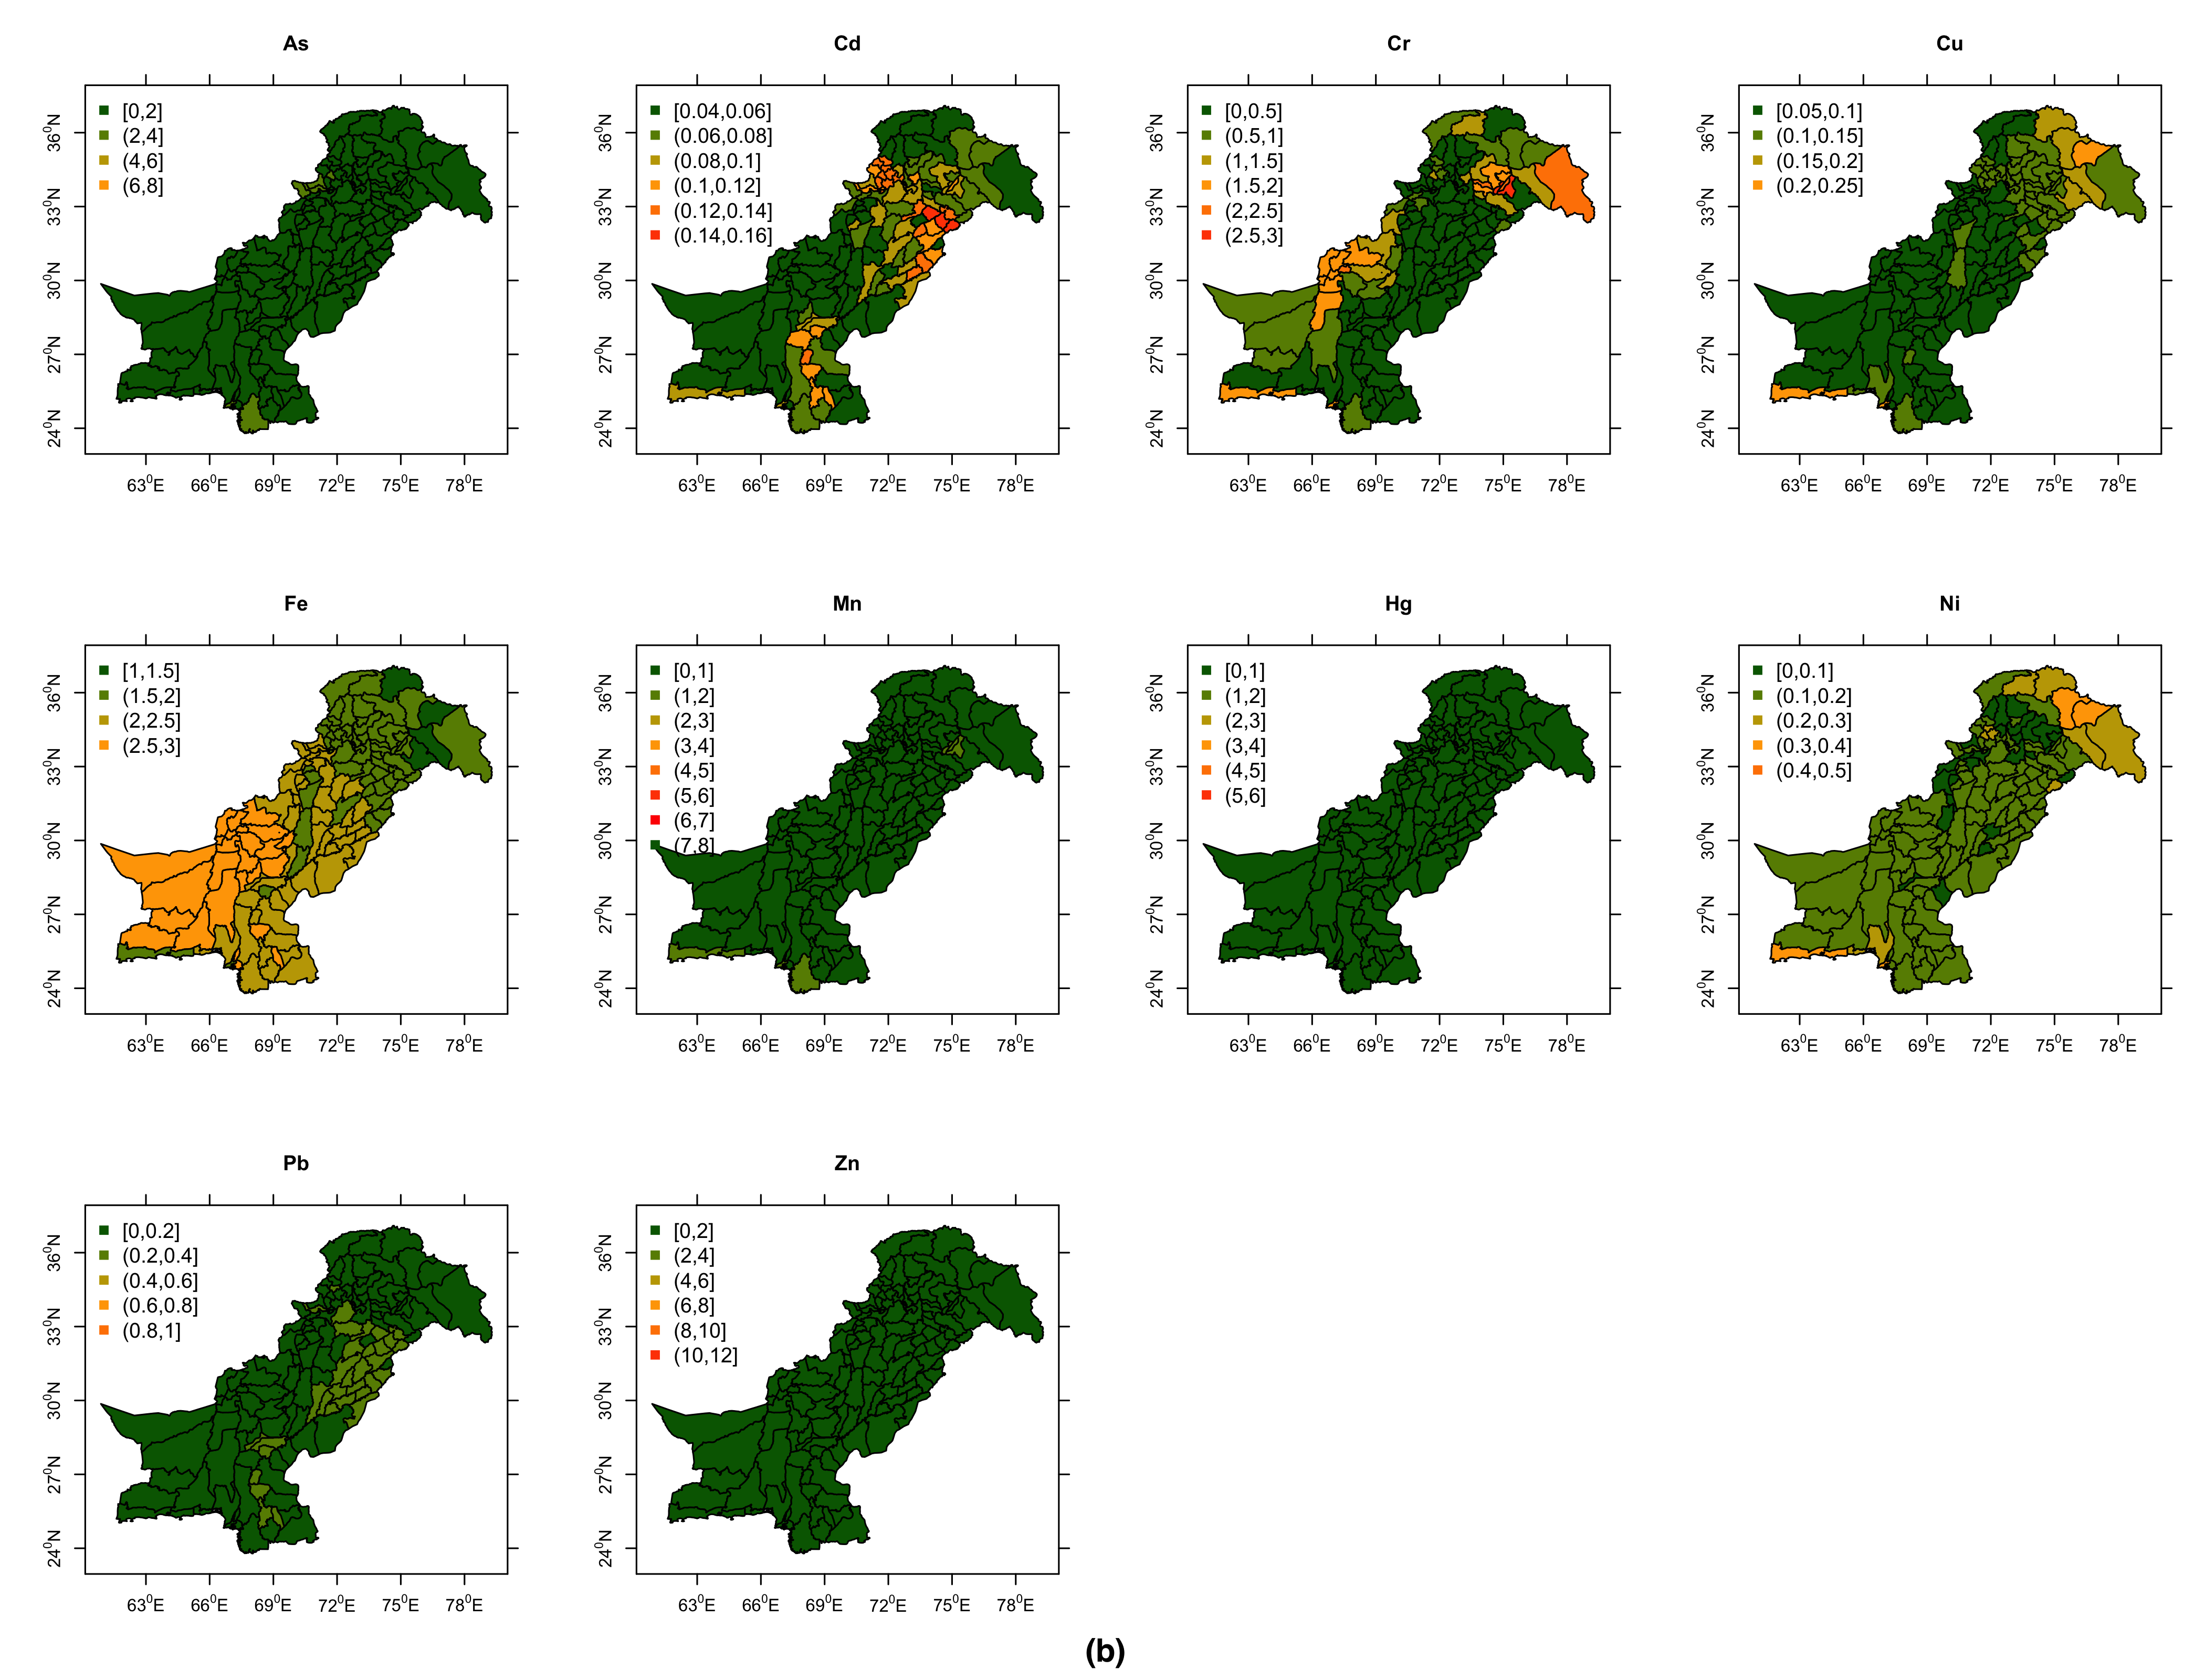
\includegraphics[width=\linewidth]{Figures/Fig_D_4_b.png}
  \caption{Upper confidence boundaries of GWR model predicted trace metal concentrations (in mg / l) within 95 \% confidence interval, i.e. predicted concentrations + 1.96 * standard errors, in (a) ground and (b) surface water at the districts of Pakistan. The abbreviations used: As = Arsenic, Cd = Cadmium, Cr = Chromium, Cu = Copper, Fe = Iron, Mn = Manganese, Hg = Mercury, Nickel = Ni, Pb = Lead, Zn = Zinc.}
  \label{Fig_D_4_b}
\end{figure}

\end{landscape}

\newpage

\begin{figure*}[hp!]
  \centering
  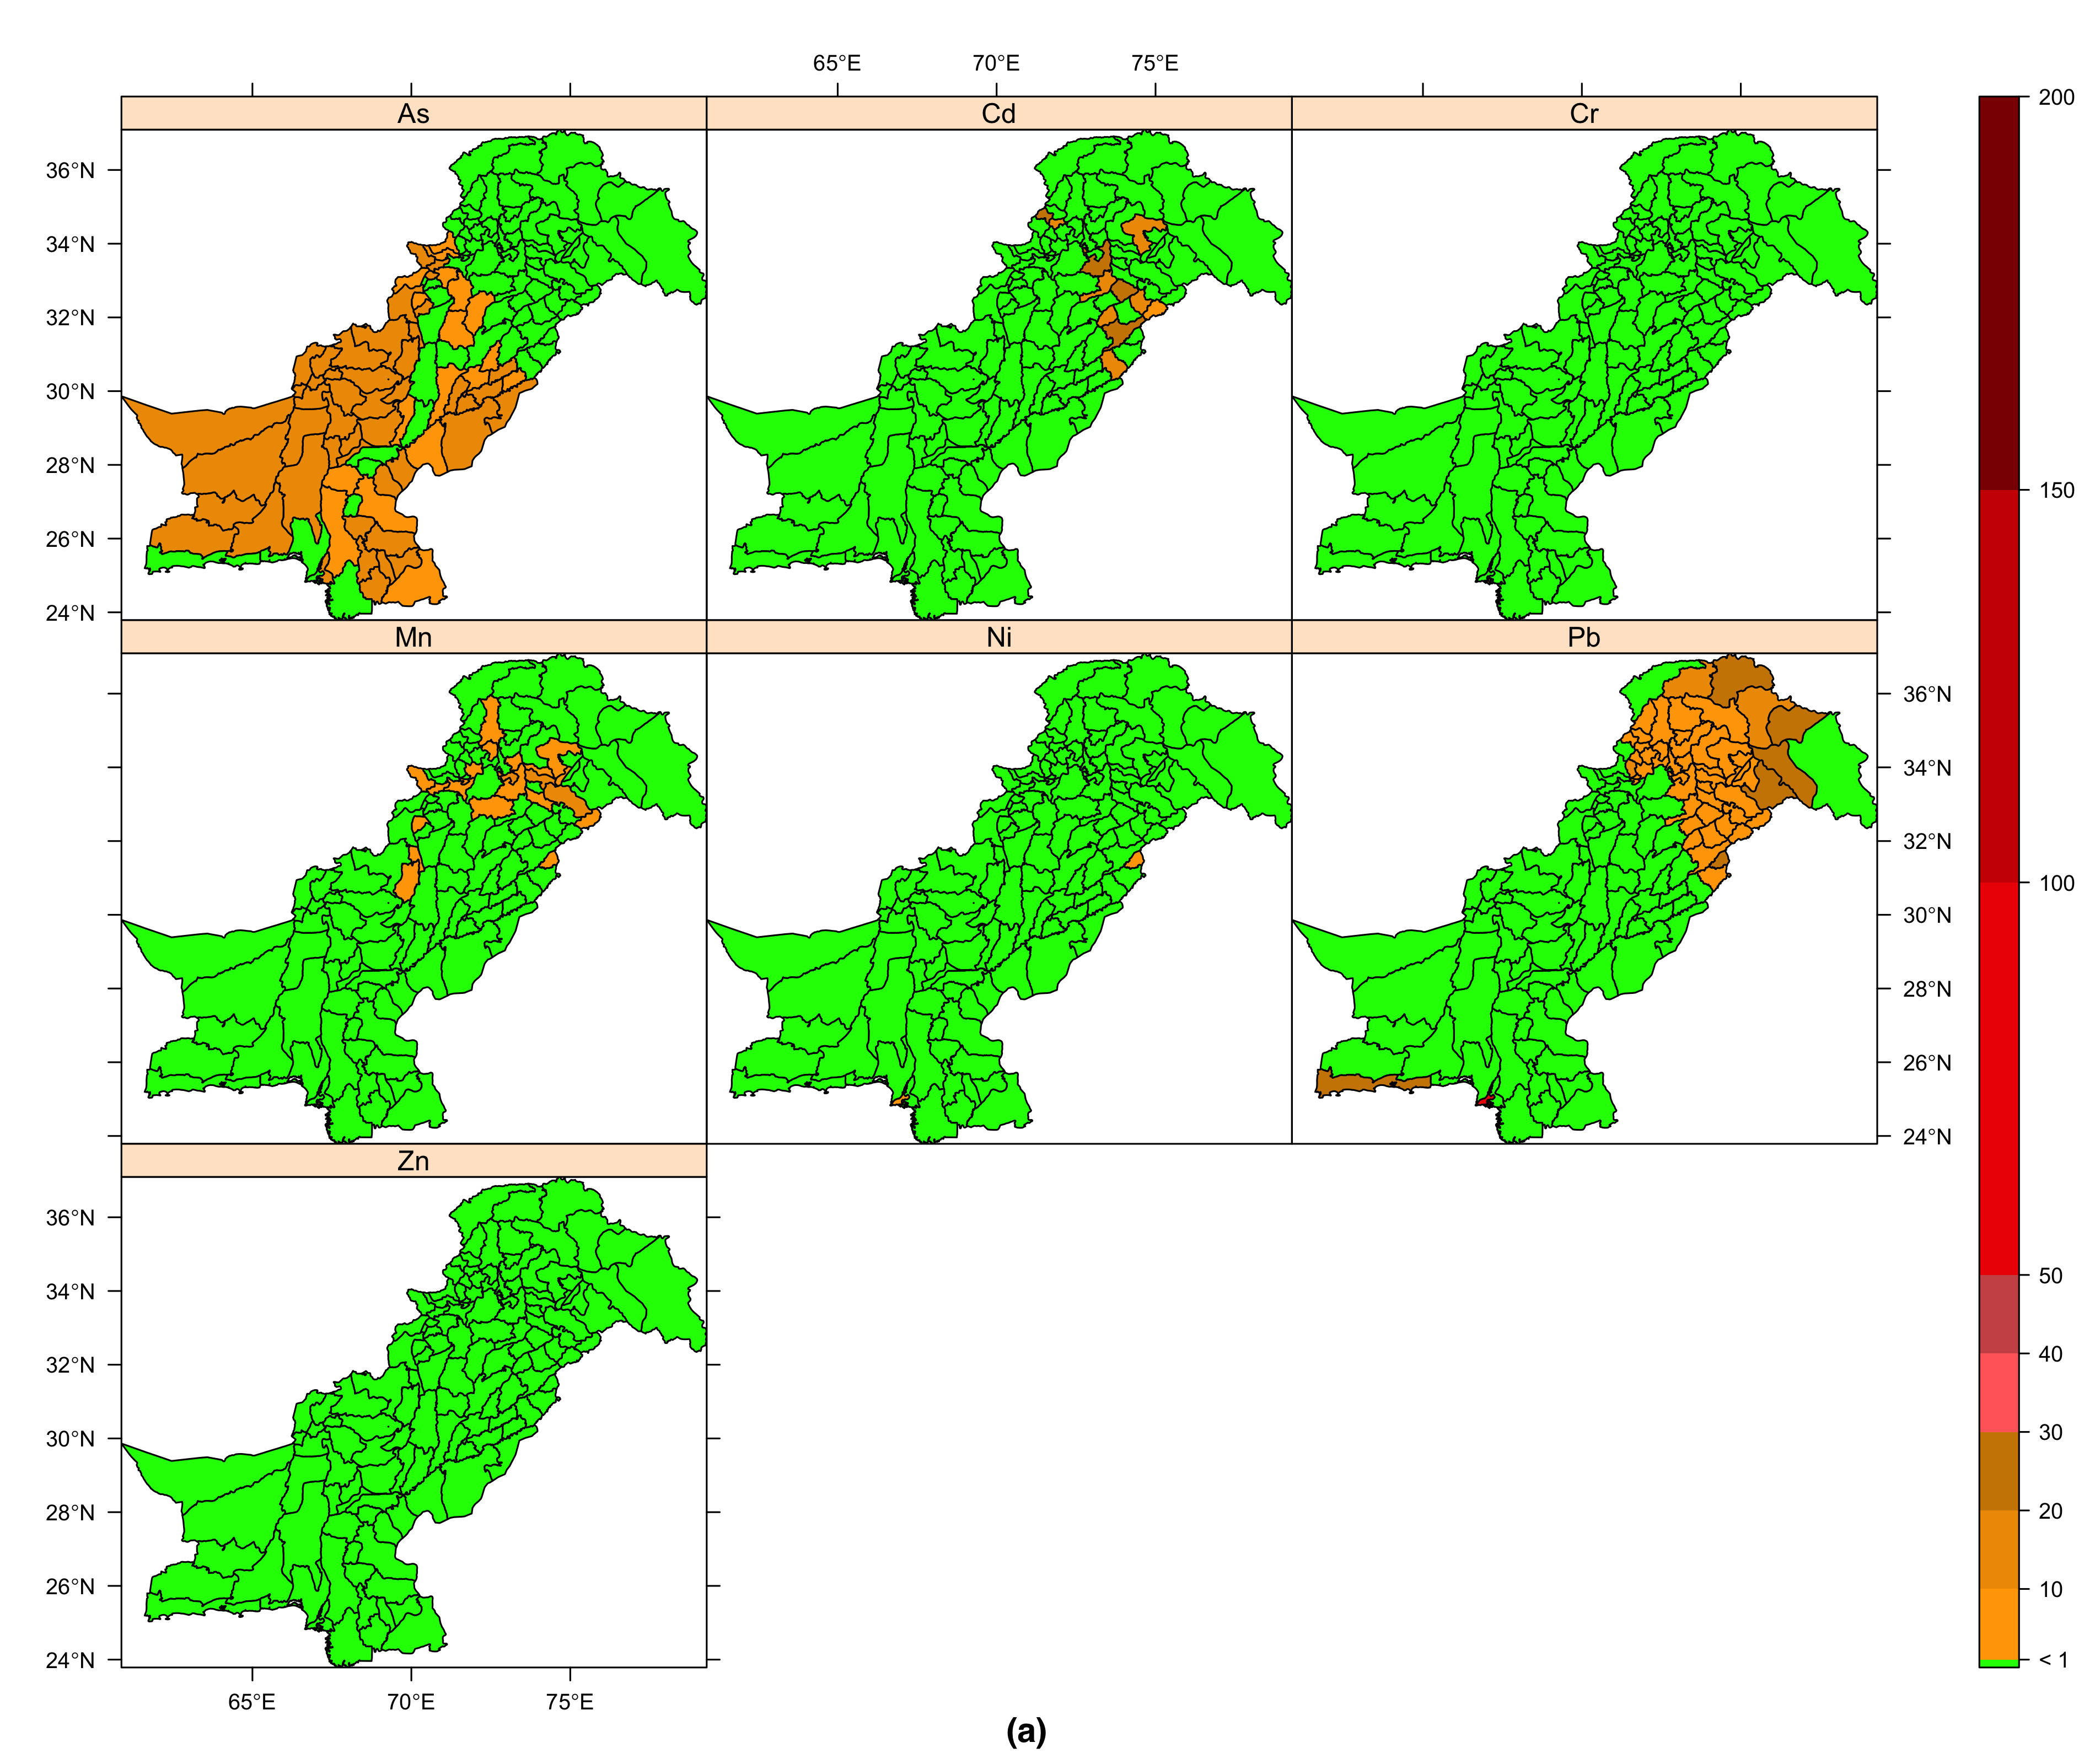
\includegraphics[width=1.1\textwidth]{Figures/Fig_D_5_a.png}
  \label{Fig_D_5_a}
\end{figure*}

\newpage

\begin{figure}[hp!]
  \centering
  \captionsetup{width=1.1\textwidth}
  \hspace{-2cm} 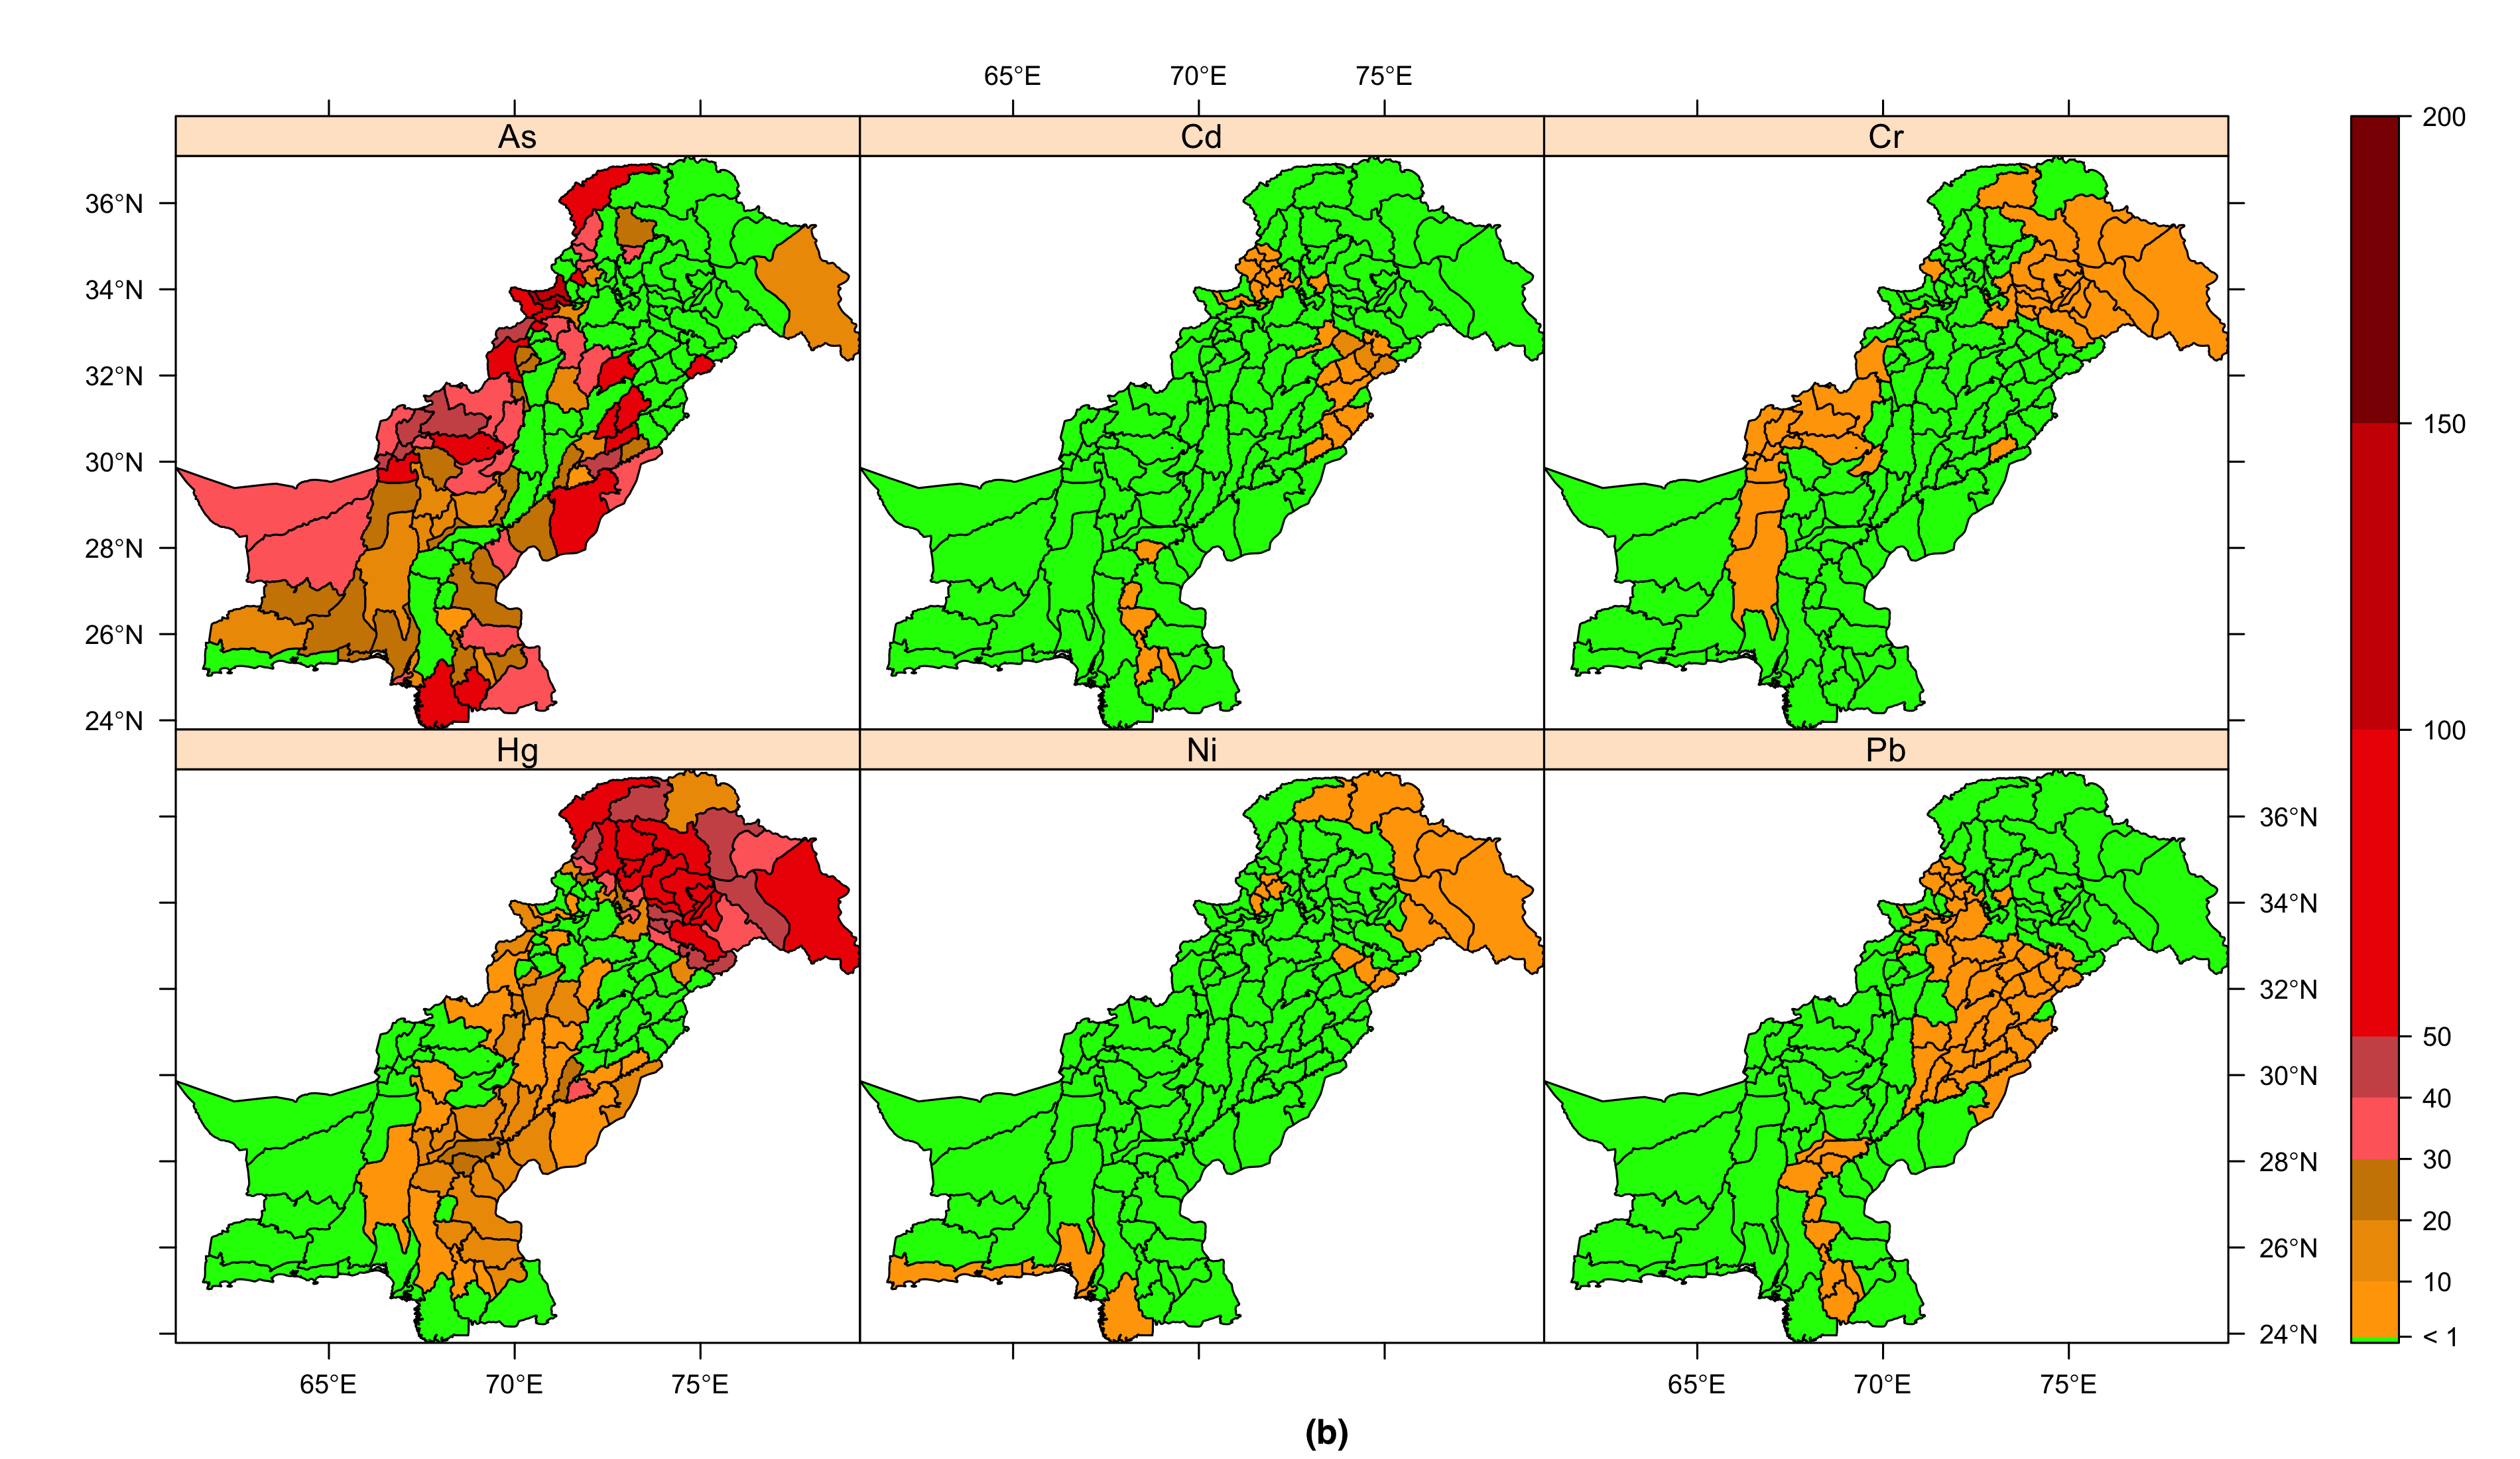
\includegraphics[width=1.1\textwidth]{Figures/Fig_D_5_b.png}
  \caption{Predicted risks, i.e. exceedances of threshold concentrations in risk quotients (RQ), for the lower confidence boundaries of GWR model predicted trace metal concentrations within 95 \% confidence interval, i.e. predicted concentrations – 1.96 * standard errors, in (a) ground and (b) surface water at the districts of Pakistan. Green indicates no exceedance, i.e. RQ $\leq$ 1. The abbreviations used: As = Arsenic, Cd = Cadmium, Cr = Chromium, Cu = Copper, Fe = Iron, Mn = Manganese, Hg = Mercury, Nickel = Ni, Pb = Lead, Zn = Zinc. Maps of Cu and Fe for ground water, and Cu, Fe, Mn and Zn for surface water are omitted because no risky district was found, i.e. for none of the districts RQ $>$ 1.}
  \label{Fig_D_5_b}
\end{figure}

\newpage

\begin{figure*}[hp!]
  \centering
  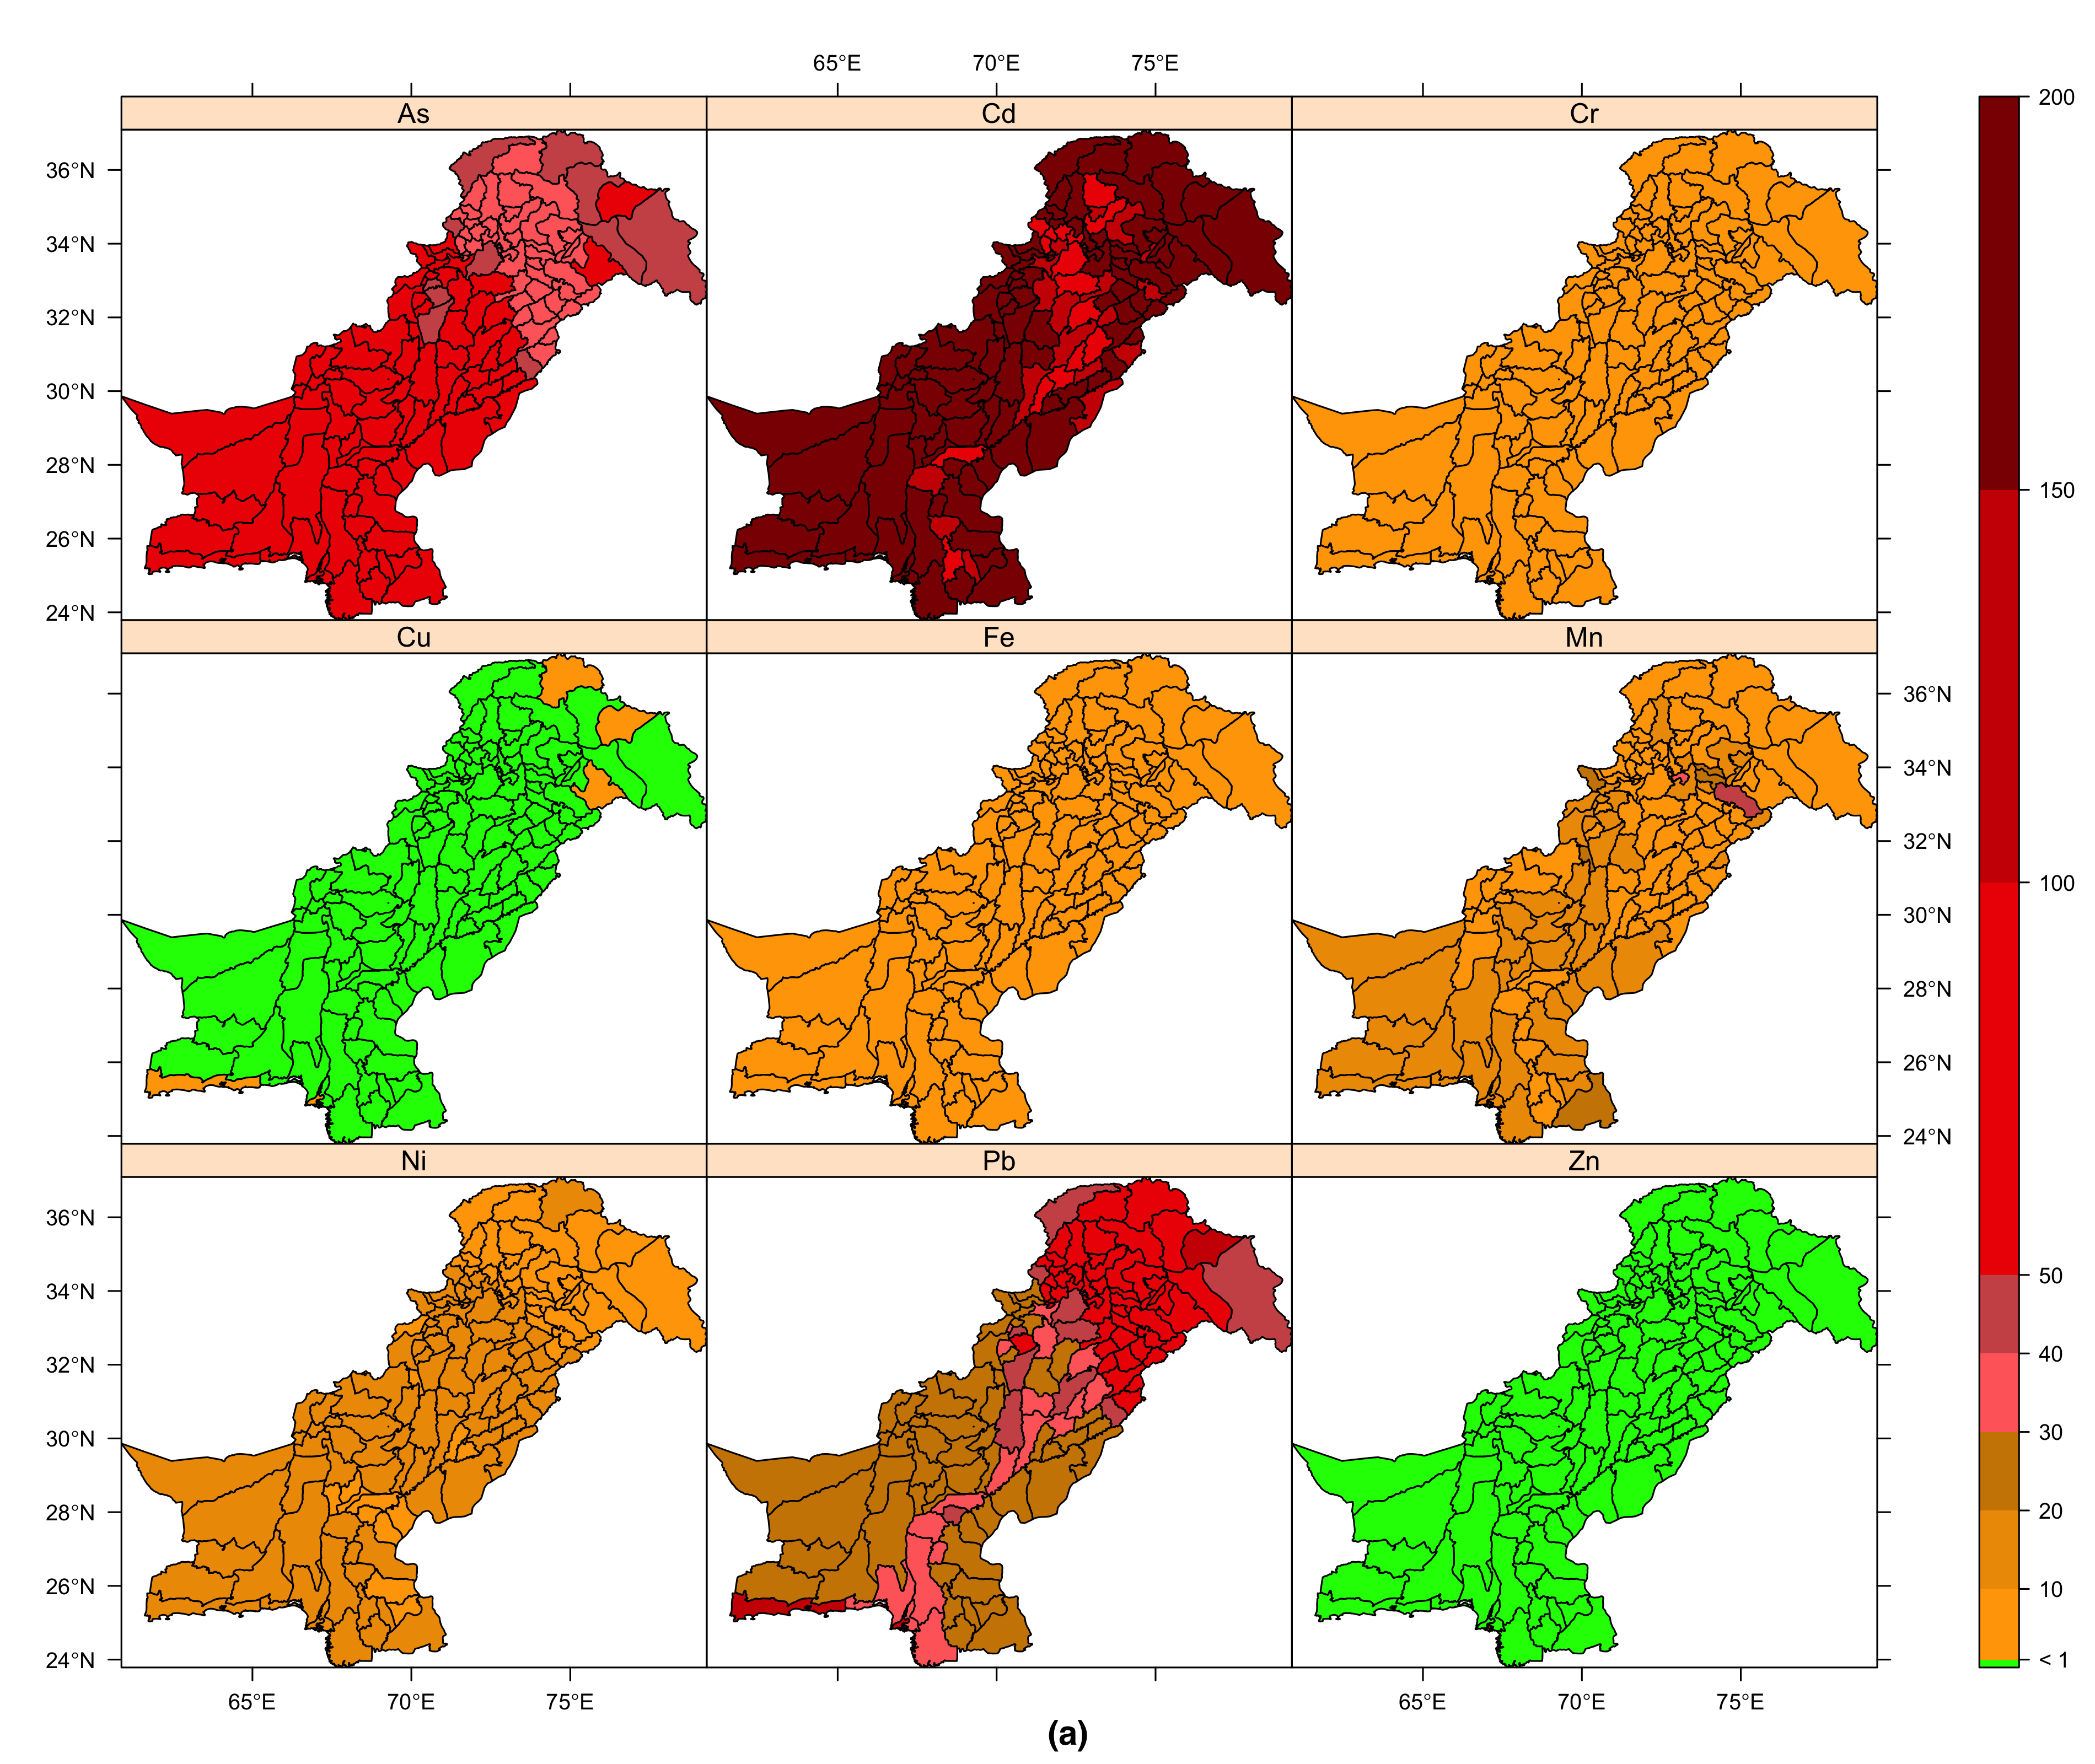
\includegraphics[width=1.1\textwidth]{Figures/Fig_D_6_a.png}
  \label{Fig_D_6_a}
\end{figure*}

\newpage

\begin{figure}[hp!]
  \centering
  \captionsetup{width=1.1\textwidth}
  \hspace{-2.0cm} 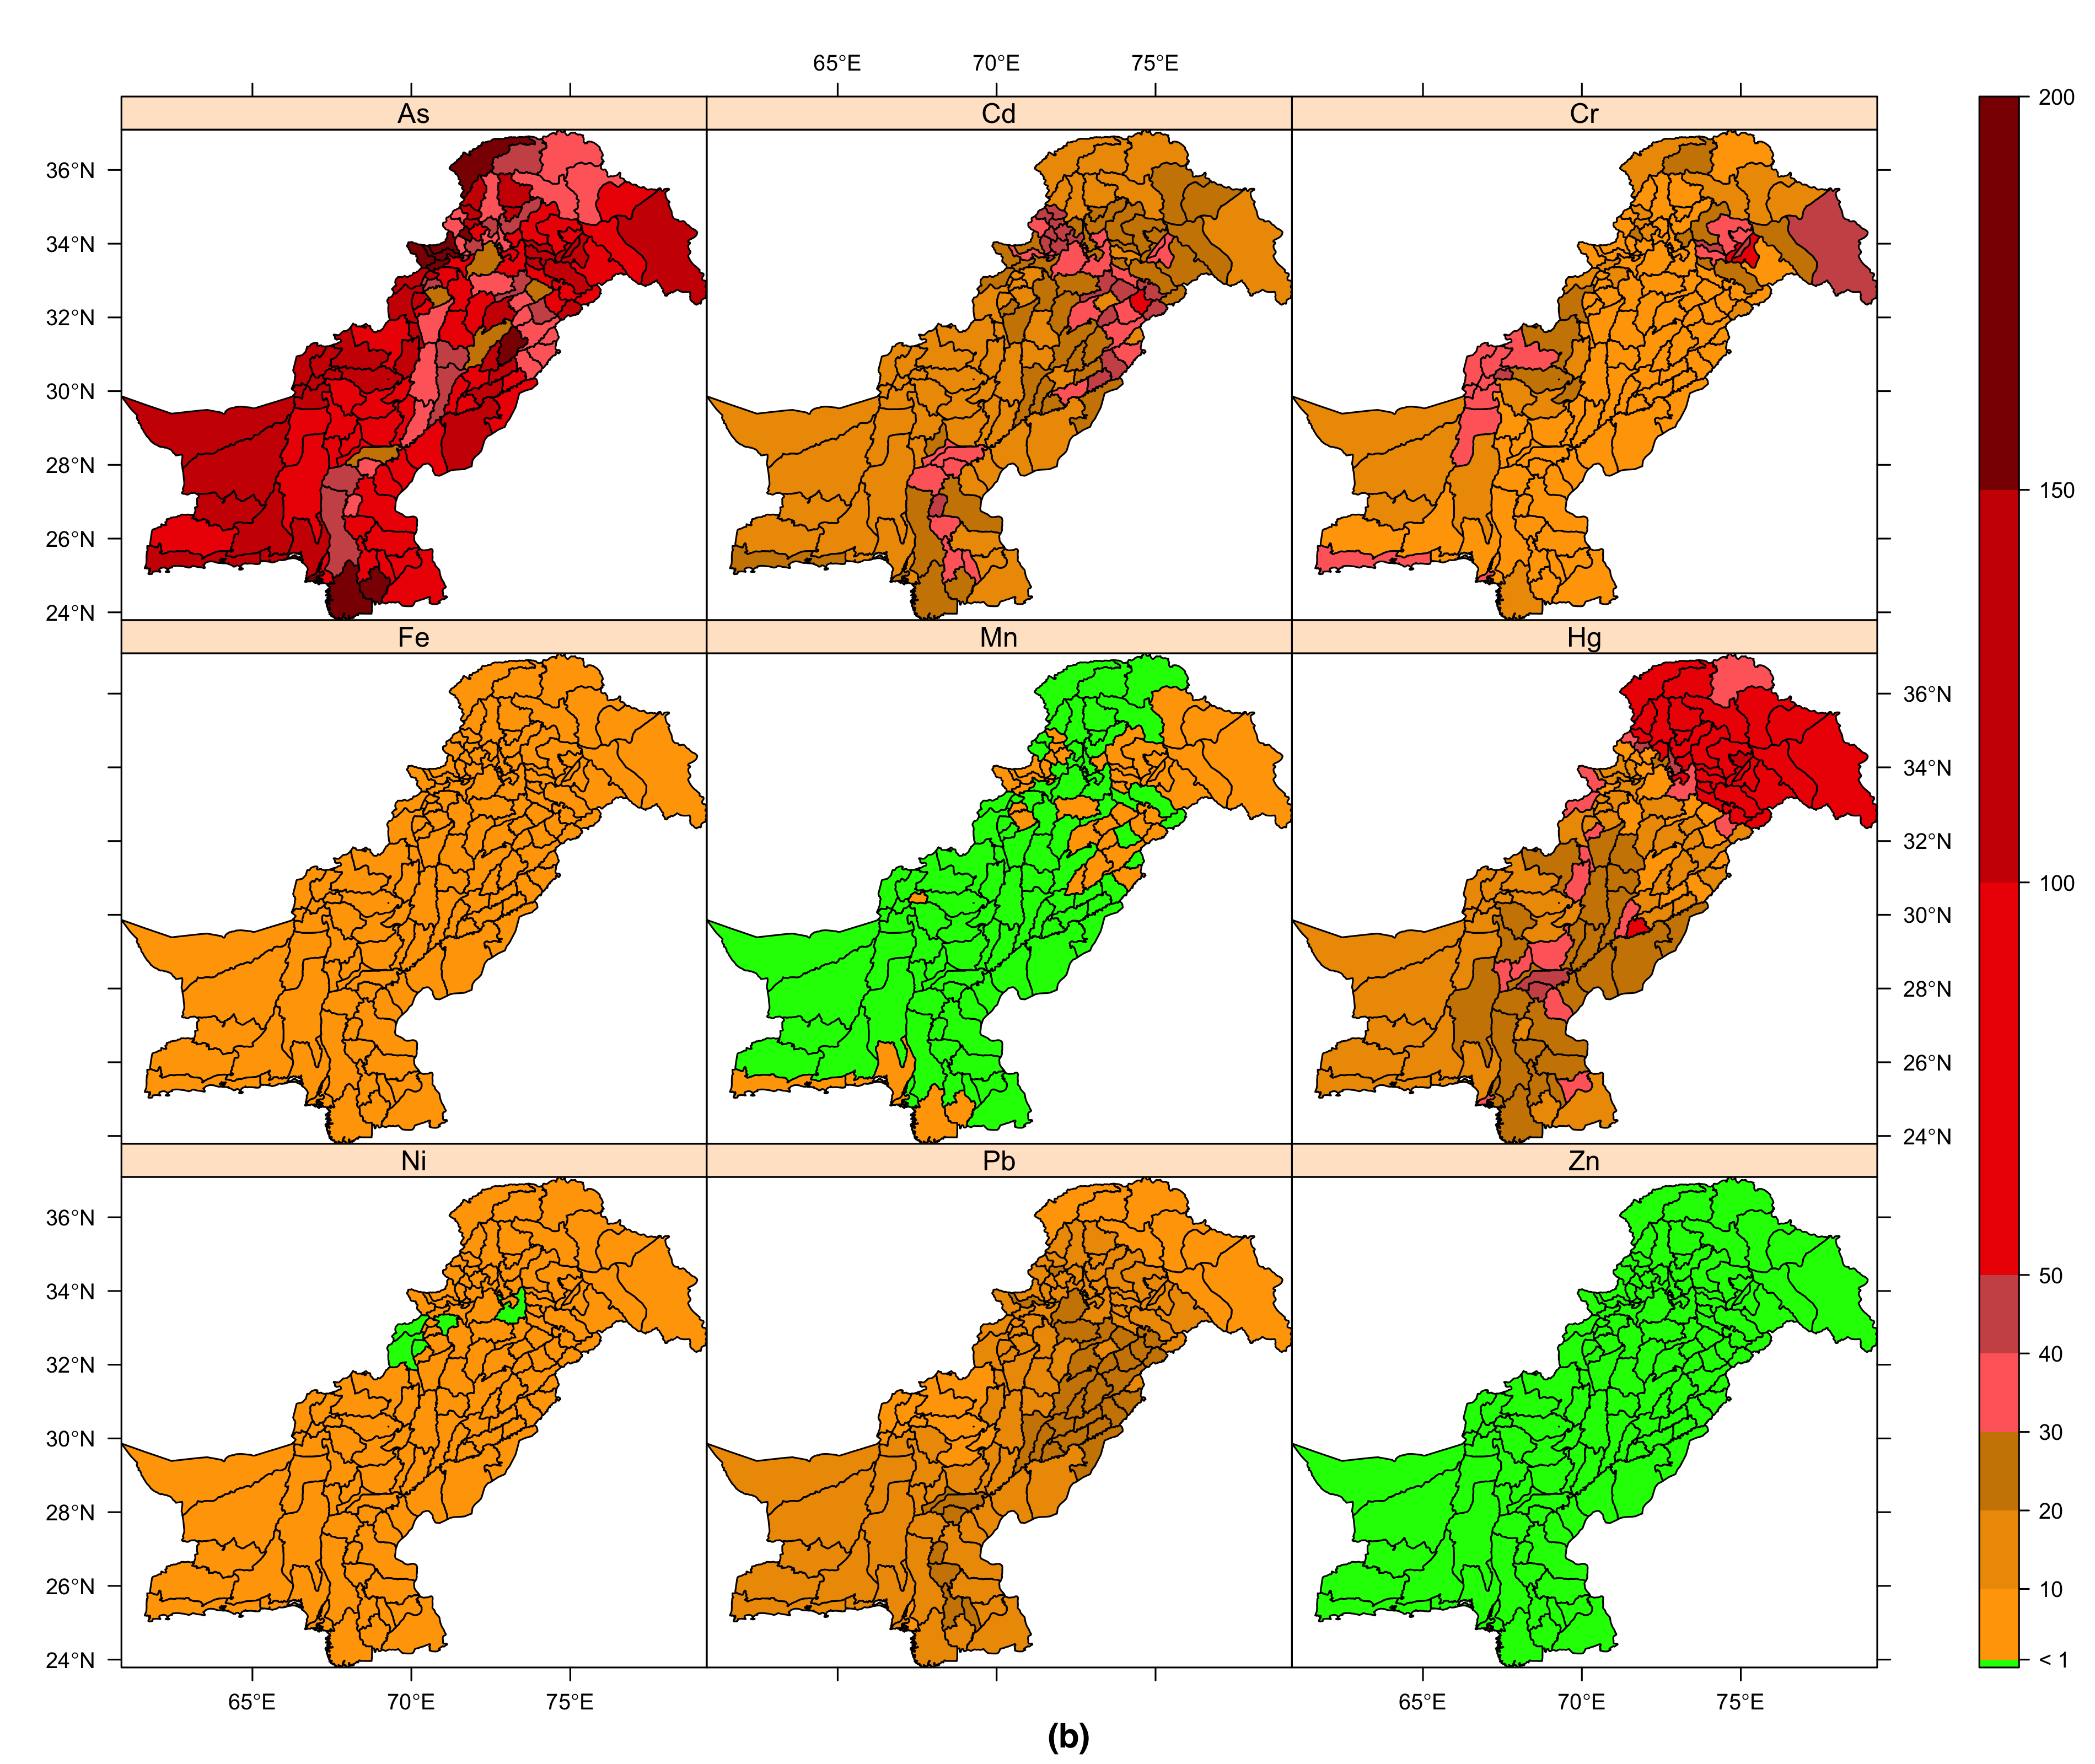
\includegraphics[width=1.1\textwidth]{Figures/Fig_D_6_b.png}
  \caption{Predicted risks, i.e. exceedances of threshold concentrations in risk quotients (RQ), for the upper confidence boundaries of GWR model predicted trace metal concentrations within 95 \% confidence interval, i.e. predicted concentrations + 1.96 * standard errors, in (a) ground and (b) surface water at the districts of Pakistan. Green indicates no exceedance, i.e. RQ $\leq$ 1. The abbreviations used: As = Arsenic, Cd = Cadmium, Cr = Chromium, Cu = Copper, Fe = Iron, Mn = Manganese, Hg = Mercury, Nickel = Ni, Pb = Lead, Zn = Zinc. Map of Cu for surface water is omitted because no risky district was found, i.e. for none of the districts RQ $>$ 1.}
  \label{Fig_D_6_b}
\end{figure}

\section{Supplementary tables}
\label{Supplementary tables}

\newpage

\begin{landscape}

\begin{table}[hp!]

\label{Table D.1}

\caption{Observed concentration values (mg / l) of the trace metals in ground water samples from different districts of Pakistan during 1997-2014. The years of observed concentrations refer to the publication years of corresponding studies.}

\centering

\begin{threeparttable}

\begin{tabular}{>{\centering\arraybackslash}m{3.3cm}>{\centering\arraybackslash}m{0.5cm}>{\centering\arraybackslash}m{0.9cm}>{\centering\arraybackslash}m{0.8cm}>{\centering\arraybackslash}m{0.9cm}>{\centering\arraybackslash}m{0.8cm}>{\centering\arraybackslash}m{0.9cm}>{\centering\arraybackslash}m{1.0cm}>{\centering\arraybackslash}m{0.9cm}>{\centering\arraybackslash}m{0.9cm}>{\centering\arraybackslash}m{0.9cm}>{\centering\arraybackslash}m{0.9cm}>{\centering\arraybackslash}m{4.4cm}}

\toprule
\textbf{Sampling location} & \textbf{n} & \multicolumn{10}{c}{\textbf{Mean concentration}} & \textbf{Study}\\
\textbf{(district)} & & \multicolumn{10}{c}{\textbf{(mg/l)}} & \\
 & & \textbf{As} & \textbf{Hg} & \textbf{Ni} & \textbf{Cu} & \textbf{Mn} & \textbf{Cr} & \textbf{Fe} & \textbf{Zn} & \textbf{Cd} & \textbf{Pb} & \\

\midrule

Lahore & 30 & 0.121 & - & - & - & - & - & - & - & - & - & Sultana et al., 2013\\
Kasur & 65 & < DL & - & 0.13 & 1.3 & 1.06 & 0.01 & 3.7 & 1.84 & < DL & 0.12 & Mahmood and Maqbool, 2006\\
Kasur  & 24 & 0.113 & - & - & - & - & - & - & - & - & - & Farooqi et al., 2007 b\\
Dera Ghazi Khan & 32 & 0.029 & - & - & - & - & - & - & - & - & - & Malana et al., 2011\\
Muzaffargarh  & 49 & 0.071 & - & - & - & - & - & - & - & - & - & Nickson et al., 2005\\
Multan & 3 & 0.53 & - & < DL & < DL & 0.53 & < DL & 1.4 & < DL & < DL & < DL & Nickson et al., 2005\\
Faislabad & 26 & < DL & - & 0.96 & 0.21 & 1.22 & 0.14 & 0.16 & 0.13 & 0.04 & 0.33 & Midrar-ul-Haq et al., 2005\\
Kalanlawala & 24 & 0.966 & - & < DL & < DL & < DL & < DL & < DL & < DL & - & < DL & Farooqi et al., 2007a\\
Sialkot & 25 & < DL & - & 0.1 & 0.06 & 0.03 & 0.03 & 0.18 & 0.16 & - & 0.49 & Ullah et al., 2009\\
Jamshoro & 45 & 0.08 & - & - & - & - & - & 0.79 & < DL & - & < DL & Baig et al., 2009\\
Therparkar & 140 & 0.75 & - & - & - & - & - & - & - & - & - & Brahman et al.,  2013\\
South East Sindh & 25 & 0.0633 & - & - & - & - & - & - & - & - & - & Kazi et al., 2009\\
Karachi & - & 0.08 & 0.01 & 0.5 & 0.09 & < DL & 0.34 & < DL & 4.02 & 0.04 & 2 & Rehman et al.,1997\\
Nowshera & 44 & < DL & 0.001 & 1.43 & 0.67 & 1.56 & 0.155 & 0.22 & 0.22 & 0.155 & 0.375 & Midrar-ul-Haq et al., 2005\\
Charsadda & 951 & < DL & < DL & 0.0094 & 0.071 & < DL & 0.0188 & 0.372 & 0.36 & 0.0053 & 0.0638 & Khan et al., 2012\\
Charsadda & 315 & - & - & 0.0007 & 0.289 & - & 0.0139 & 0.0549 & 0.135 & 0.0007 & 0.0089 & Khan et al., 2013\\
Swabi & 3 & - & - & 0.048 & 0.893 & 0.16 & 0.128 & 0.0205 & 0.0205 & 0.016 & 0.705 & Nasrullah et al., 2006\\
Peshawar & 4 & - & - & 0.88 & 0.36 & 0.12 & 0.089 & 0.143 & 0.131 & 0.03 & 0.66 & Tariq et al., 2006\\
Kohistan & 37 & 0.0021 & - & - & - & - & - & 0.327 & - & - & - & Muhammad et al., 2010\\
Kohistan & 10 & - & - & 0.0001 & 0.077 & 0.0013 & 2E-05 & - & 0.262 & 0.0001 & 0.0007 & Muhammad et al., 2011\\
Mohamnd Agency & 51 & - & - & 0.04 & 2.4 & 0.3 & 0.2 & 0.05 & 0.024 & 0.0006 & 0.0009 & Shah et al., 2012\\
Shiekhupura & - & 0.39 & - & - & 0.21 & 0.28 & - & - & - & 0.36 & - & Qazi et al., 2014\\

\bottomrule

WHO drinking water effect-threshold & & 0.01 & 0.001 & 0.02 & 2 & 0.5 & 0.05 & 0.3 & 3 & 0.003 & 0.01 & WHO, 2011\\
\hline

\end{tabular}
\begin{tablenotes}
\footnotesize
n= number of sites, As = Arsenic, Cd = Cadmium, Cr = Chromium, Cu = Copper, Fe = Iron, Mn = Manganese, Hg = Mercury, Nickel = Ni, Pb = Tin, Zn = Zinc, - = not sampled or not known, DL = detection limit, WHO=World Health Organization.
\end{tablenotes}
\end{threeparttable}
\end{table}

\clearpage

\begin{table}[hp!]

\label{Table D.2}

\vspace{-1.3cm} 

\caption{Observed concentration values (mg / l) of the trace metals in surface water samples from different districts of Pakistan during 1991-2014. The years of observed concentrations refer to the publication years of corresponding studies.}

\centering

\begin{threeparttable}

\begin{tabular}{>{\centering\arraybackslash}m{3.3cm}>{\centering\arraybackslash}m{0.5cm}>{\centering\arraybackslash}m{0.9cm}>{\centering\arraybackslash}m{0.8cm}>{\centering\arraybackslash}m{0.9cm}>{\centering\arraybackslash}m{0.8cm}>{\centering\arraybackslash}m{0.9cm}>{\centering\arraybackslash}m{1.0cm}>{\centering\arraybackslash}m{0.9cm}>{\centering\arraybackslash}m{0.9cm}>{\centering\arraybackslash}m{0.9cm}>{\centering\arraybackslash}m{0.9cm}>{\centering\arraybackslash}m{4.2cm}}

\toprule
\textbf{Sampling location} & \textbf{n} & \multicolumn{10}{c}{\textbf{Mean concentration}} & \textbf{Study}\\
\textbf{(district)} & & \multicolumn{10}{c}{\textbf{(mg/l)}} & \\
 & & \textbf{As} & \textbf{Hg} & \textbf{Ni} & \textbf{Cu} & \textbf{Mn} & \textbf{Cr} & \textbf{Fe} & \textbf{Zn} & \textbf{Cd} & \textbf{Pb} & \\

\midrule

Islamabad & 50 & - & - & - & 0.017 & 0.013 & 0.097 & 0.076 & 0.0132 & 0.0075 & 0.0446 & Iqbal et al., 2014\\
Mohmand Agency & 51 & - & - & 0.1052 & 0.06 & 0.35 & 0.32 & 0.158 & 0.0128 & 0.0005 & 0.001 & Shah et al., 2012\\
Kohistan & 18 & 0.0007 & - & - & - & - & - & 0.447 & - & - & - & Muhammad et al., 2010\\
Kohistan & 8 & - & - & 0.0003 & 0.082 & 0.0005 & 0.0001 & - & 0.015 & 0.0001 & 0.0003 & Muhammad et al., 2011\\
Islamabad  & 30 & - & - & 0.51 & 0.08 & 0.26 & 1.17 & 30.04 & 3.45 & 0.06 & 0.41 & Malik et al., 2010\\
Mianwali & - & 0.75 & 0.017 & 0.065 & 0.004 & 0.004 & 0.071 & 0.004 & 0.029 & 0.003 & 0.058 & Ashraf et al., 1991\\
Mianwali & - & - & - & 0.127 & - & - & - & - & 0.174 & - & - & Tariq et al., 1996\\
Muzaffargarh & 30 & 0.0011 & 0.053 & 0.127 & 0.011 & 0.016 & 0.018 & 1.548 & 0.01 & 0.016 & 0.125 & Tariq et al., 1995\\
Muzaffargarh & 25 & 0.007 & < DL & - & - & 0.28 & - & 0.18 & - & - & - & Nickson et al., 2005\\
Sukhar & 12 & 0.62 & 0.14 & 0.061 & 0.004 & 0.018 & 0.002 & 0.012 & 0.028 & 0.002 & 0.107 & Ashraf et al., 1991\\
Lahore & 45 & 0.0018 & 0.0006 & 0.00125 & 0.006 & 0.0055 & 0.0009 & 0.0845 & 0.022 & 0.0008 & 0.001 & Tariq et al., 1994\\
Lahore & - & - & - & 0.93 & 0.45 & 0.85 & 0.07 & 8 & 1.7 & 0.18 & 0.03 & Kashif et al., 2009\\
Kalar Kahar  & 25 & - & - & 0.0325 & 0.006 & - & - & 2.83 & 1.63 & 0.03 & 0.155 & Raza et al., 2007\\
Sehwan & 20 & - & - & 0.0027 & 0.0084 & - & - & 0.0151 & 0.0057 & 0.0091 & 0.0068 & Mastoi et al., 2008\\
Manchar Lake & 80 & 0.102 & - & 0.0043 & 0.0089 & - & - & 0.0012 & 0.0157 & 0.001 & 0.009 & Mastoi et al., 2008\\
Manchar Lake & 160 & 0.0811 & - & 0.017 & 0.019 & 0.0732 & 0.0075 & 3 & 3 & 0.0108 & 0.0833 & Kazi et al., 2009\\
Jamshoro & 45 & 0.042 & - & - & - & - & - & 0.19 & 1.489 & - & - & Baig et al., 2009\\
Jamshoro & 58 & 0.075 & - & - & - & - & - & 2.34 & - & - & - & Arain et al., 2009(b)\\
Besham & - & - & - & 0.253 & - & - & - & - & 0.016 & - & - & Tariq et al., 1996\\
Chagai & - & - & - & 0.096 & - & - & - & - & 0.028 & - & - & Tariq et al., 1996\\
Khushalgarh & - & - & - & 0.075 & - & - & - & - & 0.018 & - & - & Tariq et al., 1996\\
Dera Gazi Khan & - & - & - & 0.124 & - & - & - & - & 0.172 & - & - & Tariq et al., 1996\\
Gilgit & 22 & 0.0025 & 0.135 & 0.245 & 0.091 & 0.013 & 0.017 & 0.041 & 0.011 & 0.002 & 0.013 & Tariq et al., 1995\\
Jacobabad & 34 & 0.0008 & 0.21 & 0.124 & 0.04 & 0.015 & 0.034 & 0.034 & 0.011 & 0.011 & 0.038 & Tariq et al., 1995\\
Sialkot & 40 & 0.0013 & 0.208 & 0.124 & 0.026 & 0.209 & 0.018 & 0.209 & 0.062 & 0.014 & 0.073 & Tariq et al., 1996\\
Sialkot & - & - & - & 0.1 & 0.2 & - & - & 0.8 & 0.1 & 0.3 & 0.2 & Qadir et al., 2008\\

\bottomrule

WHO drinking water effect-threshold & & 0.01 & 0.001 & 0.02 & 2 & 0.5 & 0.05 & 0.3 & 3 & 0.003 & 0.01 & WHO, 2011\\
\hline

\end{tabular}
\begin{tablenotes}
\footnotesize
n= number of sites, As = Arsenic, Cd = Cadmium, Cr = Chromium, Cu = Copper, Fe = Iron, Mn = Manganese, Hg = Mercury, Nickel = Ni, Pb = Tin, Zn = Zinc, - = not sampled or not known, DL = detection limit, WHO = World Health Organization.
\end{tablenotes}
\end{threeparttable}
\end{table}

\end{landscape}

\begingroup

\renewcommand{\addcontentsline}[3]{}

\begin{thebibliography}

\bibitem{} \hangindent=1cm Arain, MB, Kazi TG, Baig JA, Jamali MK, Afridi HI,Shah AQ, Jalbani N, Sarfraz RA. Determination of arsenic levels in lake water, sediment, and foodstuff from selected area of Sindh, Pakistan: estimation of daily dietary intake. Food Chem Toxicol 2009; l47: 242-248.

\bibitem{} \hangindent=1cm Ashraf M, Tariq J, Jaffar M. Contents of trace metals in fish, sediment and water from three freshwater reservoirs on the Indus River, Pakistan. Fish Res 1991;12: 355–64.

\bibitem{} \hangindent=1cm Azizullah A, Khattak MNK, Richter P, Haider  D. Water pollution in Pakistan and its impact on public health — A review. Environ Int 2011; 37: 479–497.

\bibitem{} \hangindent=1cm Baig JA, Kazi TG, Arain MB, Afridi HI, Kandhro GA, Sarfraz RA, Jamali MK, Shah AQ.  Evaluation of arsenic and other physico-chemical parameters of surface and ground water of Jamshoro, Pakistan. J Hazard Mater 2009; 166: 662-669.

\bibitem{} \hangindent=1cm Brahman, KD, Kazi, TG, Afridi HI, Naseem S, Arain SS,  Ullah N. Evaluation of high levels of fluoride, arsenic species and other physicochemical parameters in underground water of two sub districts of Tharparkar, Pakistan: a multivariate study. Water Res 2013, 47: 1005–1020.

\bibitem{} \hangindent=1cm Farooqi A, Masuda H, Kusakabe M,Naseem M , Firdous N. Distribution of highly arsenic and fluoride contaminated groundwater from east Punjab, Pakistan, and the controlling role of anthropogenic pollutants in the natural hydrological cycle. Geochem J 2007; 41: 213 – 234.

\bibitem{} \hangindent=1cm Farooqi A, Masuda H, Siddiqui R, Naseem M. Sources of arsenic and fluoride in highly contaminated soils causing groundwater contamination in Punjab, Pakistan. Arch Environ Contam Toxicol 2008; 56(4): 693-706.

\bibitem{} \hangindent=1cm Iqbal J, Shah MH. Occurrence, risk assessment, and source apportionment of heavy metals in surface sediments from Khanpur Lake, Pakistan. J Analytical Sci Tech 2014; 5(1): 28. doi: 10.1186/s40543-014-0028-z.

\bibitem{} \hangindent=1cm Kashif SR, Akram M, Yaseen M, Ali S. Studies on heavy metals status and their uptake by vegetables in adjoining areas of Hudiara drain in Lahore. Soil and Environ 2009, 28(1): 7-12, 

\bibitem{} \hangindent=1cm Kazi TG, Arain MB, Baig JA, Jamali MK, Afridi HI, Jalbani N, Sarfraz RA, Shah AQ, Niaz A. The correlation of arsenic levels in drinking water with the biological samples of skin disorders. Sci Total Environ 2009; 407:1019–1025.

\bibitem{} \hangindent=1cm Khan S, Shahnaz M, Jehan N, Rehman S, Shah MT, Din I. Drinking water quality and human health risk in Charsadda district, Pakistan. J Cleaner Prod 2012; 3: 60:93-101.

\bibitem{} \hangindent=1cm Mahmood S, Maqbool A. Impacts of wastewater irrigation on water quality and on the health of local community in Faisalabad. Pak J Water Res 2006; 10: 19–22.

\bibitem{} \hangindent=1cm Malana MA, Khosa MA. Groundwater pollution with special focus on arsenic, Dera Ghazi Khan-Pakistan. J Saudi Chem Soc 2011; 15: 39–47.

\bibitem{} \hangindent=1cm Malik RN, Nadeem M. Spatial and temporal characterization of trace elements and nutrients in the Rawal Lake Reservoir, Pakistan using multivariate analysis techniques. Environ Geochem and Health  2011; 33(6): 525-41.

\bibitem{} \hangindent=1cm Mastoi GM, Shah SGS, Khuhawar MY. Assessment of water quality of Manchar Lake in Sindh (Pakistan). Environ Monit Assess 2008; 141: 287–96.

\bibitem{} \hangindent=1cm Midrar-Ul-Haq, Khattak RA, Puno HK, Saif MS, Memon KS. Surface and ground water contamination in NWFP and Sindh provinces with respect to trace elements. Int J Agri Biol 2005; 7:214–227.

\bibitem{} \hangindent=1cm Muhammad S, Shah MT, Khan S. Arsenic health risk assessment in drinking water and source apportionment using multivariate statistical techniques in Kohistan region, northern Pakistan. Food Chem Toxicol 2010; 48:2855–2864

\bibitem{} \hangindent=1cm Muhammad S, Shah MT, Khan S. Health risk assessment of heavy metals and their source apportionment in drinking water of Kohistan region, northern Pakistan. Microchem J 2011; 98:334–343.

\bibitem{} \hangindent=1cm Nasrullah, Naz R, Bibi H, qbal M, Durrani MI. Pollution load in industrial effluent and ground water of Gadoon Amazai Induatrial Estate (GAIE) Swabi, NWFP. J Agri Biol Sci 2006; 1:18–24.

\bibitem{} \hangindent=1cm Nickson R, McArthur JM, Shrestha B, Kyaw-Myint TO, Lowry D. Arsenic and other drinking water quality issues, Muzaffargarh District, Pakistan. Appl Geochem 2005; 20: 5-68.

\bibitem{} \hangindent=1cm Qadir A, Malik RN, Hussain SZ. Spatio-temporal variations in water quality of Nullah Aik-tributary of the river Chenab, Pakistan. Environ Monit Assess 2008; 140:43-59.

\bibitem{} \hangindent=1cm Qazi MA, Khattak MA, Khan MSA, Chaudhry MN, Mahmood K , Akhter B, Iqbal N, Ilyas S, Ali UA. Sptial Distribution of the heavy metals in the gorund water of Shiekhupura distirct, Punjab, Pakistan. J Agric Res 2014; 52(1):99-110.

\bibitem{} \hangindent=1cm Rahman A, Lee HK, Khan MA. Domestic water contamination in rapidly growing mega cities of Asia: case of Karachi, Pakistan. Environ Monit Assess 1997; 44:339–60.

\bibitem{} \hangindent=1cm Raza N, Niazi SB, Sajid M, Iqbal F, Ali M. Studies on relationship between season and inorganic elements of Kallar Kahar Lake (Chakwal), Pakistan. Journal of Research (Science), Bahauddin Zakariya University, Multan, Pakistan 2007;18:61–8.

\bibitem{} \hangindent=1cm Shah MT, Ara J, Muhammad S, Khan S, Tariq S. Health risk assessment via surface water and sub-surface water consumption in the mafic and ultramafic terrain, Mohmand agency, northern Pakistan. J Geochem Explor 2012; 118: 60–67

\bibitem{} \hangindent=1cm Sultana J,  Abida F,  Usman A. Arsenic concentration variability, health risk assessment, and source identification using multivariate analysis in selected villages of public water system, Lahore, Pakistan. Environ Monit Assess 2014; 186:1241–1251. 

\bibitem{} \hangindent=1cm Tariq J, Ashraf M, Jaffar M, Afzal M.Pollution status of the Indus River, Pakistan, through heavy metal and macronutrient contents of fish, sediment and water. Water Res 1996; 30:1337-1344.

\bibitem{} \hangindent=1cm Tariq J, Jaffar M, Ashraf M. Trace metal concentration, distribution and correlation in water, sediment and fish from the Ravi River, Pakistan. Fish Res 1994; 19:131–149.

\bibitem{} \hangindent=1cm Tariq M. Ali M,Shah Z. Characteristics of industrial effluents and their possible impacts on quality of underground water. Soil Environ 2006; 25: 64–79.

\bibitem{} \hangindent=1cm Ullah R,  Malik RN, Qadir A. Assessment of Groundwater Contamination in an Industrial City, Sialkot, Pakistan. Afr. J. Environ. Sci. Technol 2009; 3:429-446.

\bibitem{} \hangindent=1cm World Health Organization, 2011. Guidelines for drinking-water quality. World Health Organization, Geneva.


\end{thebibliography}

\endgroup